%---------------------------------------------------------------------
%
%                         Project Name:Njust LabReport
%
%---------------------------------------------------------------------
%
%                 created by Qingyun Fang <fqy2017@gmail.com>
%
%                        Last-modified: 2017-6-12
%
%---------------------------------------------------------------------

\documentclass[a4paper,12pt]{report}



\usepackage{ctex}
%\usepackage{xeCJK}
\usepackage{times}
\usepackage{setspace}
\usepackage{fancyhdr}
\usepackage{float}
\usepackage{graphicx}
\usepackage{wrapfig}
\usepackage{array}
\usepackage{fontspec,xunicode,xltxtra}
\usepackage{titlesec}
\usepackage{titletoc}
\usepackage[titletoc]{appendix}
\usepackage[top=30mm,bottom=30mm,left=20mm,right=20mm]{geometry}
\usepackage{cite}
\usepackage{listings}
\usepackage[framed,numbered,autolinebreaks,useliterate]{mcode} % 插入代码
\XeTeXlinebreaklocale "zh"
\XeTeXlinebreakskip = 0pt plus 1pt minus 0.1pt

%---------------------------------------------------------------------
%	页眉页脚设置
%---------------------------------------------------------------------
\fancypagestyle{plain}{
	\pagestyle{fancy}      %改变章节首页页眉
}

\pagestyle{fancy}
\lhead{\kaishu~软件设计与开发实践报告~}
\rhead{\kaishu~1150310607~张宁~}
\cfoot{\thepage}

%---------------------------------------------------------------------
%	章节标题设置
%---------------------------------------------------------------------
%\titleformat{\chapter}{\centering\zihao{-1}\heiti}{实验\chinese{chapter}}{1em}{}
\titleformat{\chapter}{\centering\zihao{-1}\heiti}{}{1em}{}
\titlespacing{\chapter}{0pt}{*0}{*6}

%---------------------------------------------------------------------
%	摘要标题设置
%---------------------------------------------------------------------
\renewcommand{\abstractname}{\zihao{-3} 摘\quad 要}

%---------------------------------------------------------------------
%	参考文献设置
%---------------------------------------------------------------------
\renewcommand{\bibname}{\zihao{2}{\hspace{\fill}参\hspace{0.5em}考\hspace{0.5em}文\hspace{0.5em}献\hspace{\fill}}}

%---------------------------------------------------------------------
%	引用文献设置为上标
%---------------------------------------------------------------------
\makeatletter
\def\@cite#1#2{\textsuperscript{[{#1\if@tempswa , #2\fi}]}}
\makeatother

%---------------------------------------------------------------------
%	目录页设置
%---------------------------------------------------------------------
\titlecontents{chapter}[0em]{\songti\zihao{-4}}{\thecontentslabel\ }{}
{\hspace{.5em}\titlerule*[4pt]{$\cdot$}\contentspage}
\titlecontents{section}[2em]{\vspace{0.1\baselineskip}\songti\zihao{-4}}{\thecontentslabel\ }{}
{\hspace{.5em}\titlerule*[4pt]{$\cdot$}\contentspage}
\titlecontents{subsection}[4em]{\vspace{0.1\baselineskip}\songti\zihao{-4}}{\thecontentslabel\ }{}
{\hspace{.5em}\titlerule*[4pt]{$\cdot$}\contentspage}


\begin{document}
%---------------------------------------------------------------------
%	封面设置
%---------------------------------------------------------------------
\begin{titlepage}
	\begin{center}
		
    
\includegraphics[width=0.3\textwidth]{figure//sf1.png}\\
    \vspace{10mm}
    \textbf{\zihao{2}\kaishu{计算机科学与技术}}\\[0.8cm]
    \textbf{\zihao{2}\kaishu{ 软件设计与开发实践实验报告}}\\[3cm]

	\vspace{\fill}
	
\setlength{\extrarowheight}{3mm}
{\songti\zihao{3}	
\begin{tabular}{rl}
	
	{\makebox[4\ccwd][s]{班\qquad 级:}}& ~\kaishu 英才班\\
	
	{\makebox[4\ccwd][s]{姓\qquad 名:}}& ~\kaishu 张宁 \\

    {\makebox[4\ccwd][s]{学\qquad 号:}}& ~\kaishu 1150310607 \\

	{\makebox[4\ccwd][s]{指导老师:}} & ~\kaishu 曲明成\\

\end{tabular}
 }\\[2cm]
\vspace{\fill}
\zihao{4}
%2016\textasciitilde 2017第一学期\\
%使用\LaTeX 撰写于\today
	\end{center}	
\end{titlepage}

%---------------------------------------------------------------------
%  摘要页
%---------------------------------------------------------------------
\begin{abstract}
\begin{spacing}{1.5}
	{\zihao{-4}
操作系统是一种复杂的系统软件。xv6是一个运行在基于x86架构的计算机系统上的类似UNIX的教学用操作系统。xv6起源于MIT。在目前的MIT本科生课程“6.828: Operating Systems Engineering”中,xv6目前主要用于讲课.

我是在win系统上使用Oracle VM VirtualBox安装32位乌班图.

虚拟机来作为实验环境,在虚拟机上我可以使用QEMU来实现一个x86计算机, 让xv6操作系统运行在一个用软件仿真出来的x86计算机上
    \\[0.5cm]
%	\textbf{关键字}:\quad 南理工 \quad 电光院 \quad 985平台 \quad211工程
	}
\end{spacing}



\end{abstract}

%---------------------------------------------------------------------
%  目录页
%---------------------------------------------------------------------
\tableofcontents % 生成目录

%---------------------------------------------------------------------
%   xv6环境配置
%---------------------------------------------------------------------
\chapter{ xv6环境配置}

\begin{spacing}{1.5}


对于linux并不太熟悉的同学,我建议你们可以参考一些资料来快速入手一款linux操作系统, Ubuntu由于有很多用户基础,所以如果是新手的话, Ubuntu是非常不错的选择,后面的附录部分,给出了一些我觉得比较好的学习资料.
在安装完成乌班图虚拟机之后,我可以进行下一步的实验环境配置.
准备安装
\begin{lstlisting}
# 安装git   apt-get install -y git
# 安装g++apt-get install -y g++
# 安装gdbapt-get install -y gdb
# 安装编译工具链apt-get install -y build-essential
# 下载xv6的代码并且cd 到对应路径
git clone git://github.com/mit-pdos/xv6-public.git
\end{lstlisting}

\begin{figure}[H]
	\centering
	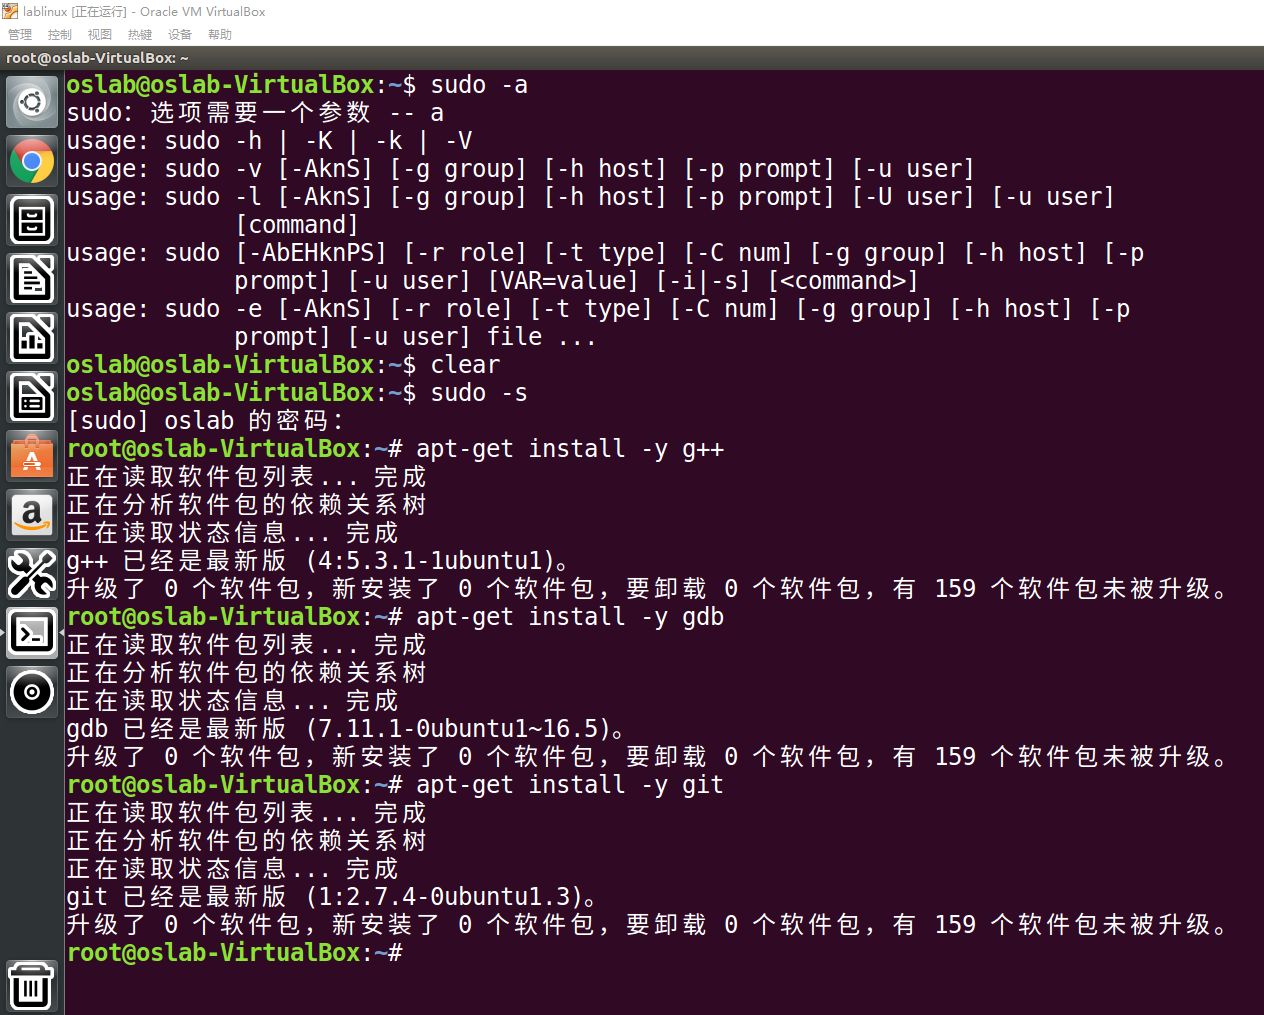
\includegraphics [width=1.0\textwidth]{figure//1.1.png}
	%\caption{}\label{dianguang13}
\end{figure}


\begin{figure}[H]
	\centering
	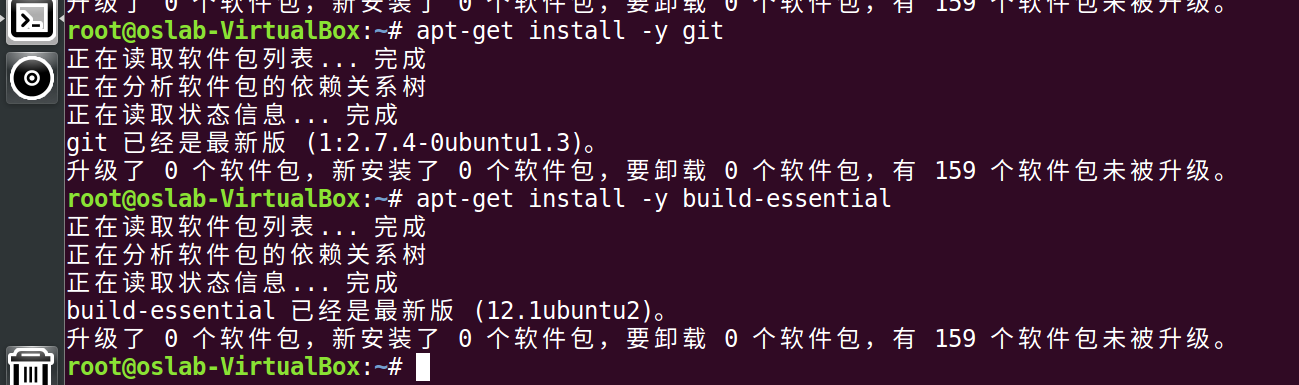
\includegraphics [width=1.0\textwidth]{figure//1.2.png}
	%\caption{}\label{dianguang13}
\end{figure}



安装qemu
\# 安装qemu apt-get install qemu

\begin{figure}[H]
	\centering
	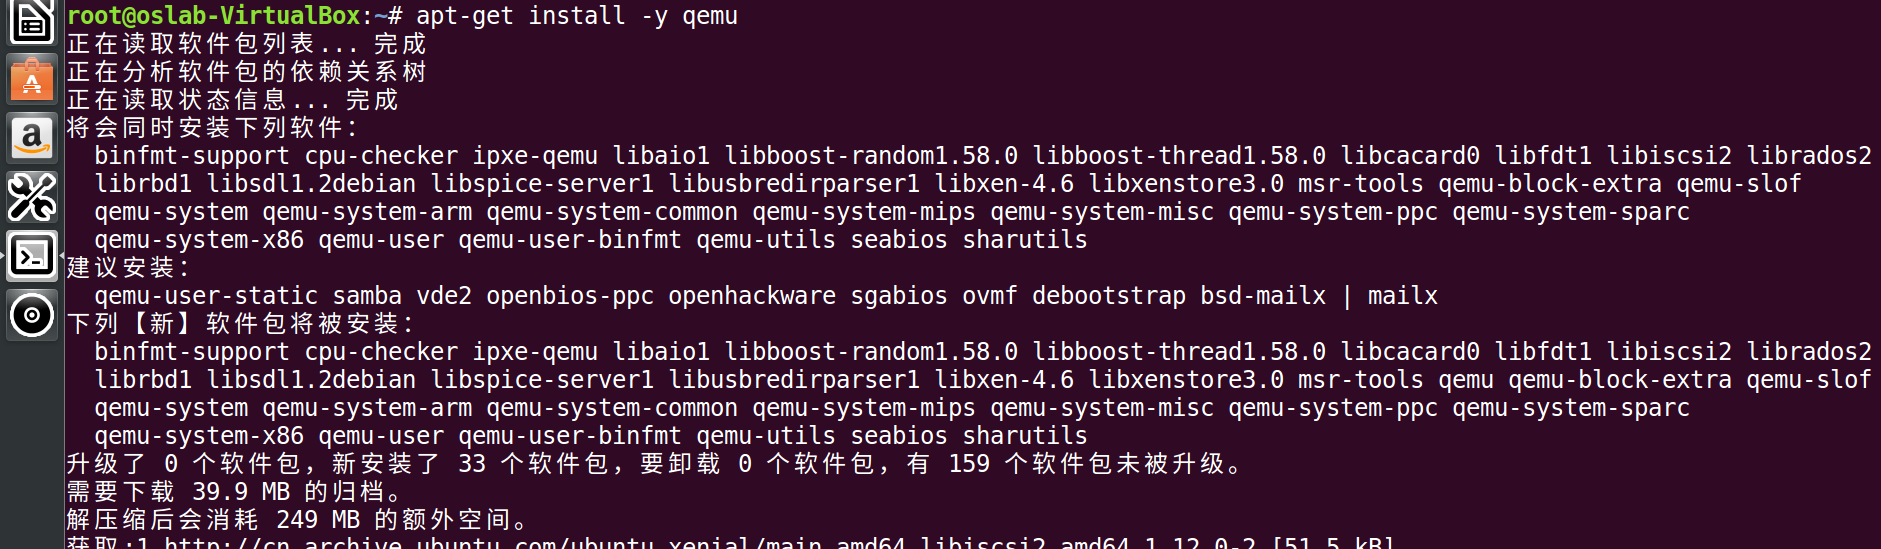
\includegraphics [width=1.0\textwidth]{figure//1.3.png}
	%\caption{}\label{dianguang13}
\end{figure}

编译xv6
cd /到对应位置/xv6-public
make qemu
生成qemu环境下运行的xv6
成功
\begin{figure}[H]
	\centering
	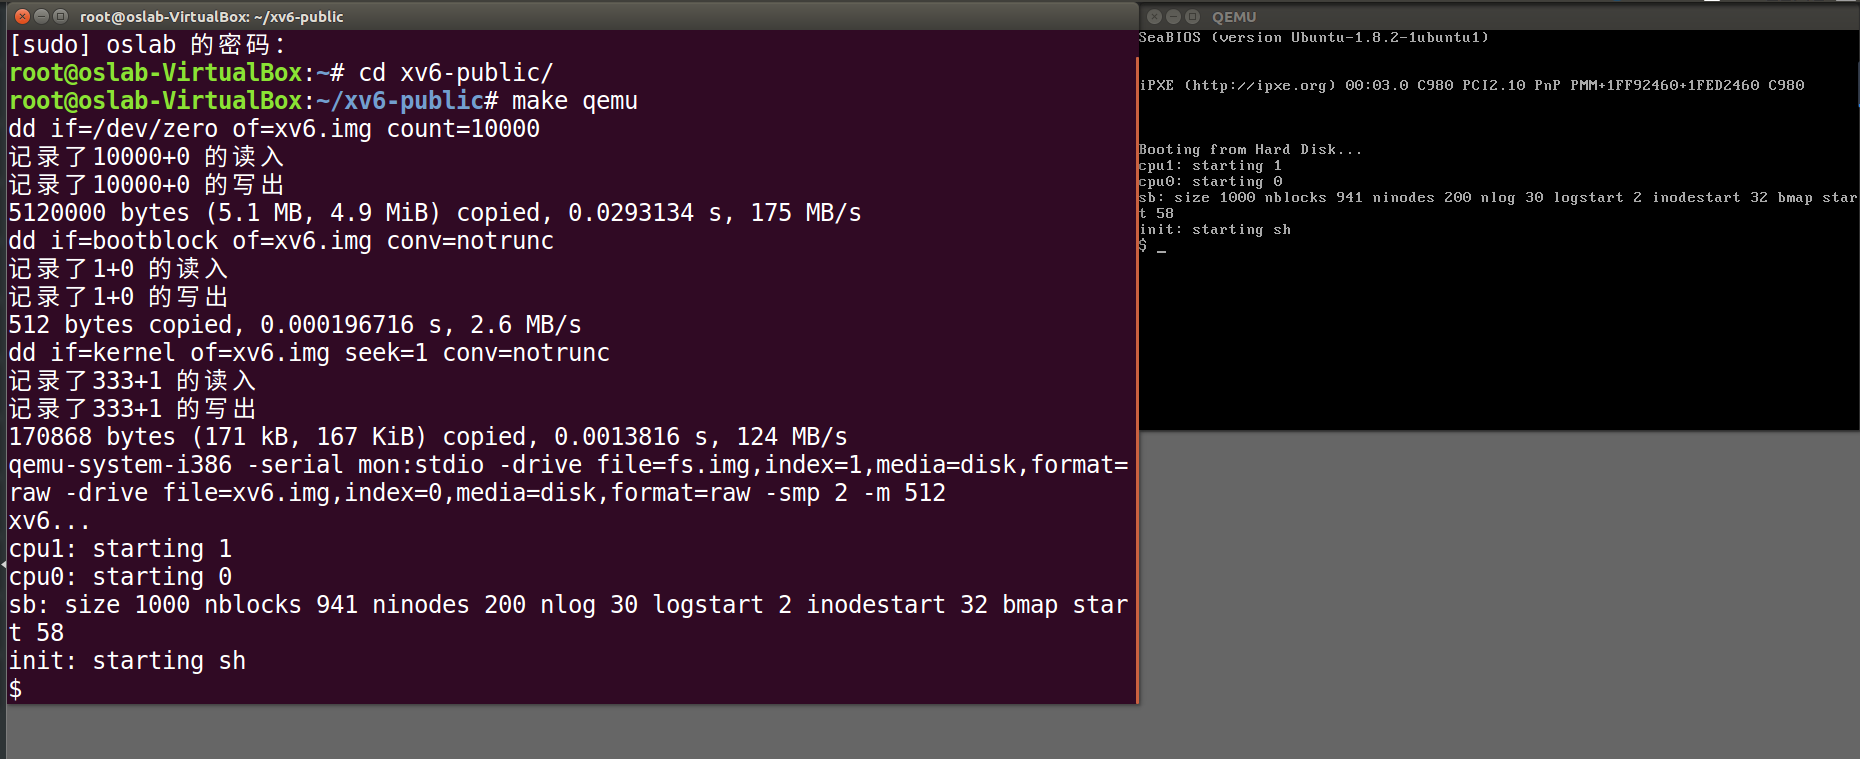
\includegraphics [width=1.0\textwidth]{figure//1.4.png}
	%\caption{}\label{dianguang13}
\end{figure}
\end{spacing}
%---------------------------------------------------------------------
%  实验一
%---------------------------------------------------------------------



%---------------------------------------------------------------------
%  实验二
%---------------------------------------------------------------------
\chapter{ Lab 2: Memory Management}


\begin{spacing}{1.5}
\section{实验目的}

\section{实验要求}

\section{实验内容}

\section{实验分析}

\end{spacing}


\chapter{ Lab 2: Memory Management}
\chapter{xv6实验系统分析}
\section{xv6的系统结构(结合示意图)}

SMP是Symmetric Multi Processing的简称,意为对称多处理计算机系统,内有许多紧耦合多处理器,这种系统的最大特点就是共享所有资源。在SMP架构中,每个处理器在功 能上都是对称、等价的。每个处理器有独自的中断处理控制器(硬件)。 内存在所有处理器之间共享。因此处理器可以通过共享的内存区域进行通讯。Xv6就是一个SMP操作系统,可以有多个cpu公共工作.
xv6基于典型的UNIX操作系统设计思路。简单地说,xv6是一种能区分内核态和用户态,基于扁平内存管理的层次型单体内核,应用程序和操作系统是处于不同的特权状态和地址空间。代表应用程序的用户态进程运行在CPU的用户态(又称非特权模式,用户模式),无法直接访问系统硬件和操作系统中的系统数据,而操作系统运行在CPU的核心态(又称特权模式,内核模式),可以访问系统硬件和核心数据。下面给出一个xv6系统结构是示意图
\begin{figure}[H]
	\centering
	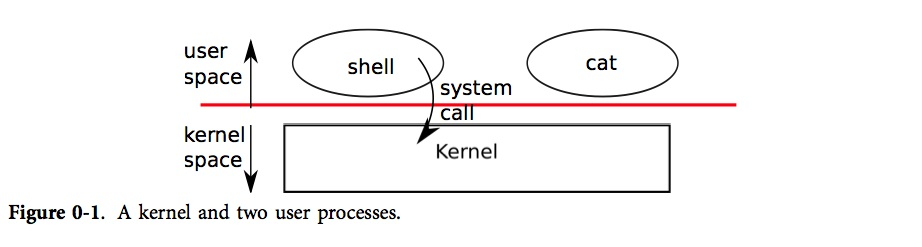
\includegraphics [width=1.0\textwidth]{figure//4.1.png}
	%\caption{}\label{dianguang13}
\end{figure}


下面分别从系统调用接口、进程/线程管理、内存管理、文件系统、I/O管理等几个方面进行总体分析。
	进程通过系统调用使用内核服务。系统调用是应用程序访问操作系统的接口。在系统调用接口上,通用操作系统与基于此操作系统的应用程序处于两个不同的CPU特权态,操作系统处于核心态,而应用程序处于用户态。在核心态可以执行CPU特权指令,而用户态无法执行特权指令,且只能通过特定的指令或中断来访问操作系统提供的各种功能。这在一定程度上保证了系统整体的安全,避免应用程序对操作系统可能的破坏。内核使用了 CPU 的硬件保护机制来保证用户进程只能访问自己的内存空间。内核拥有实现保护机制所需的硬件权限(hardware privileges),而用户程序没有这些权限。当一个用户程序进行一次系统调用时,硬件会提升特权级并且开始执行一些内核中预定义的功能。内核提供的一系列系统调用就是用户程序可见的操作系统接口,xv6 内核提供了 Unix 传统系统调用的一部分,它们是:
\begin{figure}[H]
	\centering
	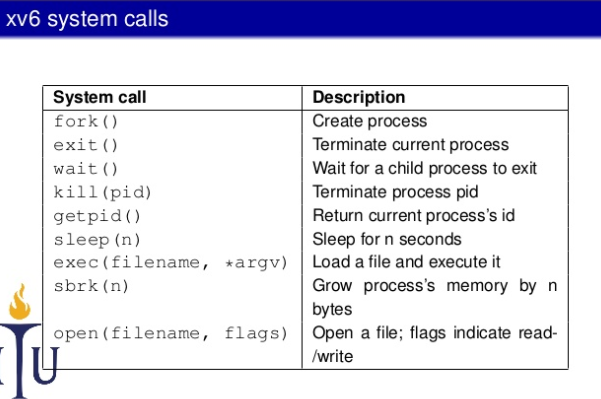
\includegraphics [width=1.0\textwidth]{figure//4.2.png}
	%\caption{}\label{dianguang13}
\end{figure}
\begin{figure}[H]
	\centering
	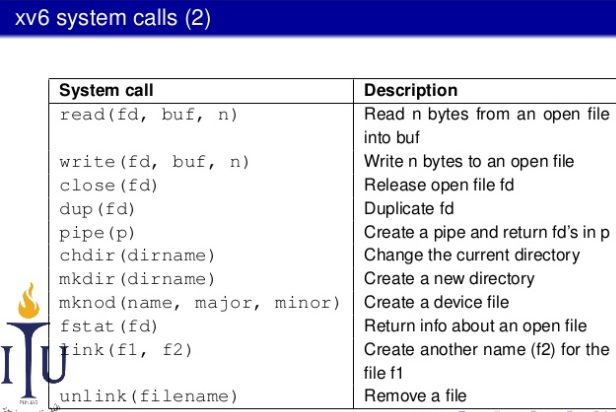
\includegraphics [width=1.0\textwidth]{figure//4.3.png}
	%\caption{}\label{dianguang13}
\end{figure}



	在内存管理方面,通用操作系统采用了虚拟内存管理方式,这样可以让内存需求超过实际物理内存的进程/线程能够执行,其主要思想是把重要和常用的数据和执行代码放在物理内存中,把不常用的数据和执行代码放到二级存储(这里主要指的是硬盘等可在掉电后保存数据的存储介质),随时根据系统执行情况替换放在内存中的数据和代码。而且通过虚存管理可以实现对不同内存区域的保护,不同进程之间,或者应用程序和操作系统之间的地址空间相对隔离。这样一般情况下不同进程的地址空间不能直接访问,且应用程序不能直接访问内核地址空间。所以一个与错误的应用程序不会导致系统的崩溃,从而增加了系统的可靠性。xv6操作系统没有采用虚拟内存管理,而是采用了简单的基于X86段模式的单一地址空间管理方式。在内存分配和释放的管理上,xv6相对实现得比较简单,采用基于可变分区分配的首次适配算法,容易产生内存碎片。
    	在进程/线程管理方面,当前通用操作系统结合虚存管理,采用进程和线程结合的管理方式。进程代表了一个程序执行的过程以及其所占用的计算机资源(包括CPU、内存、文件等),进程的执行流可用线程来表示。操作系统的调度单位可以是进程或线程。一个进程可以包含多个线程,属于同一进程的多个线程共享进程管理的资源,比如属于同一进程的多个线程共享进程所管理的内存,这样这些线程可以直接访问属于进程的全局地址空间。 xv6操作系统实现了一个基于进程(没有实现线程)的简单进程管理机制。
    	在文件系统管理方面,当前通用操作系统结合虚存管理,实现了多种复杂、高效且可靠的文件系统,且建立了一个统一的虚拟文件系统层,屏蔽不同文件系统的差异,对上层提供统一的接口。且与用户管理和进程管理结合,可实现安全管理,保证对文件的安全访问。xv6操作系统实现了一个相对简单的基于inode索引方式的文件系统。
   	在I/O管理方面,xv6操作系统与通用操作系统(特别是类UNIX操作系统)差别不是特别大,都把设备“看成”是一种特殊的设备文件,有设备号,用文件的访问接口来进行打开、关闭、读、写和控制等操作。在灵活性方面,xv6驱动程序不能象通用操作系统那样根据硬件情况动态加载,而是在编译时候就静态确定的。


\section{xv6的引导}
当计算机加电后,一般不直接执行操作系统,而是执行引导加载程序。简单地说,引导加载程序就是在操作系统内核运行之前运行的一段小程序。通过这段小程序,我可以初始化硬件设备、建立系统的内存空间映射图,从而将系统的软硬件环境带到一个合适的状态,以便为最终调用操作系统内核准备好正确的环境。最终引导加载程序把操作系统内核映像加载到RAM中,并将系统控制权传递给它。下面是一个通用操作系统的启动过程
\begin{figure}[H]
	\centering
	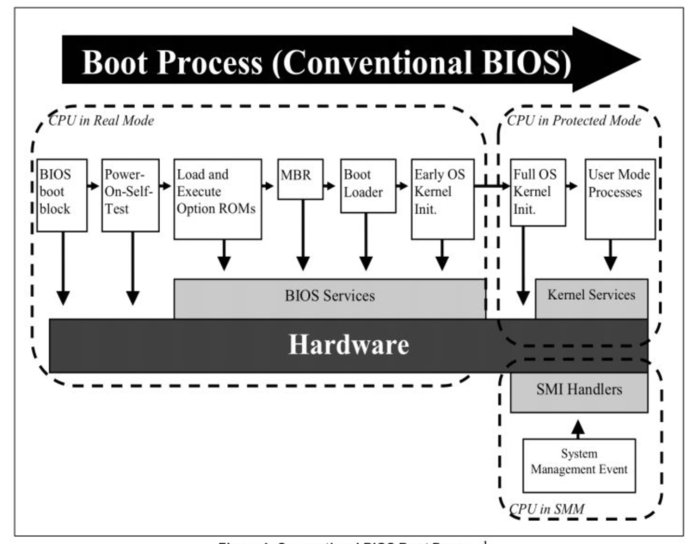
\includegraphics [width=1.0\textwidth]{figure//image87.png}
	%\caption{}\label{dianguang13}
\end{figure}
对于绝大多数计算机系统而言,操作系统和应用软件是存放在磁盘(硬盘/软盘)、光盘、EPROM、ROM、Flash等可在掉电后继续保存数据的存储介质上。计算机启动后,CPU一开始会到一个特定的地址开始执行指令,这个特定的地址存放了系统软件(不仅是操作系统,还可能是引导加载程序等)。
引导加载程序(bootloader)是系统加电后运行的第一段软件代码。对于PC386的体系结构而言,PC机中的引导加载程序由BIOS (Basic Input Output System,即基本输入/输出系统,其本质是一个固化在主板Flash/CMOS上的软件)和位于软盘/硬盘引导扇区中的OS Boot Loader一起组成。BIOS实际上是被固化在计算机ROM(只读存储器)芯片上的一个特殊的软件,为上层软件提供最底层的、最直接的硬件控制与支持。更形象地说,BIOS就是PC计算机硬件与上层软件程序之间的一个"桥梁",负责访问和控制硬件。
以PC386为例,计算机加电后,CPU从物理地址0x000FFFF0(由初始化的CS:EIP确定,此时CS和IP的值分别是0xF000和0xFFF0))开始执行。在0x000FFFF0这里只是存放了一条跳转指令,通过跳转指令跳到BIOS例行程序起始点。BIOS做完计算机硬件自检和初始化后,会选择一个启动设备(例如软盘、硬盘、光盘等),并且读取该设备的第一扇区(即启动扇区)到内存一个特定的地址0x7c00处,然后CPU控制权会转移到那个地址继续执行。至此BIOS的初始化工作做完了,进一步的工作交给了xv6。
      整个xv6系统的启动流程大致是这样的:首先BIOS将把OS的Boot Loader从磁盘上(一般是位于第一个扇区)拷贝到内存当中。当BIOS将基本的初始化程序完成后,将跳转到Boot Loader所在内存的位置继续执行。 Boot Loader将把OS的内核从磁盘上拷贝到然后运行。这样就完成了启动。
在xv6的源码中,整个启动过程主要牵涉到bootasm.S和bootmain.c两个文件

\subsection{代码分析}
bootloader代码分析
bootloader的组成
在makefile中96行~102行有如下语句
\begin{figure}[H]
	\centering
	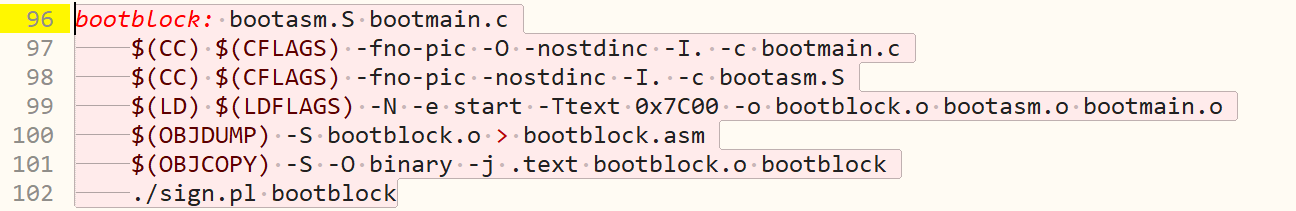
\includegraphics [width=1.0\textwidth]{figure//image88.png}
	%\caption{}\label{dianguang13}
\end{figure}
从中可以看出bootloader包含两个文件,bootasm.S和bootmain.c。生成的bootloader会写到一个主引导扇区上面。作为主引导扇区,其位置在软盘或硬盘的第一个扇区,其大小为512个字节,在此扇区的最后两个字节是一个主引导扇区特征码为”55AA”。Makefile的97行和98行是通过gcc把 bootmain.c和bootasm.S编译成目标文件bootmain.o和bootasm.o。Makefile的99行是通过ld程序把目标文件bootmain.o和bootasm.o链接成目标文件bootblock.o,且定义了起始执行的点(也称入口点)为start函数,具体的代码段起始地址为0x7C00。Makefile的100行是通过objdump程序把bootblock.o反汇编成bootlock.asm。Makefile的101行是通过objcopy程序把bootblock.o变成二进制码bootlock。Makefile的102行是通过sign.pl程序把bootlock扩展到512个字节,并把最后两个字节写成”55AA”。


bootloader的启动主要涉及到bootasm.S、bootmain.c。其中bootasm.S的主要作用是从实模式转化到保护模式。 bootmain的作用是把内核从磁盘拷贝到内存中。
bootasm.S
在进入实模式向保护模式切换之前,首先需要把中断关闭("cli" at line 13),保证转换过程不被硬件中断打断。
\begin{figure}[H]
	\centering
	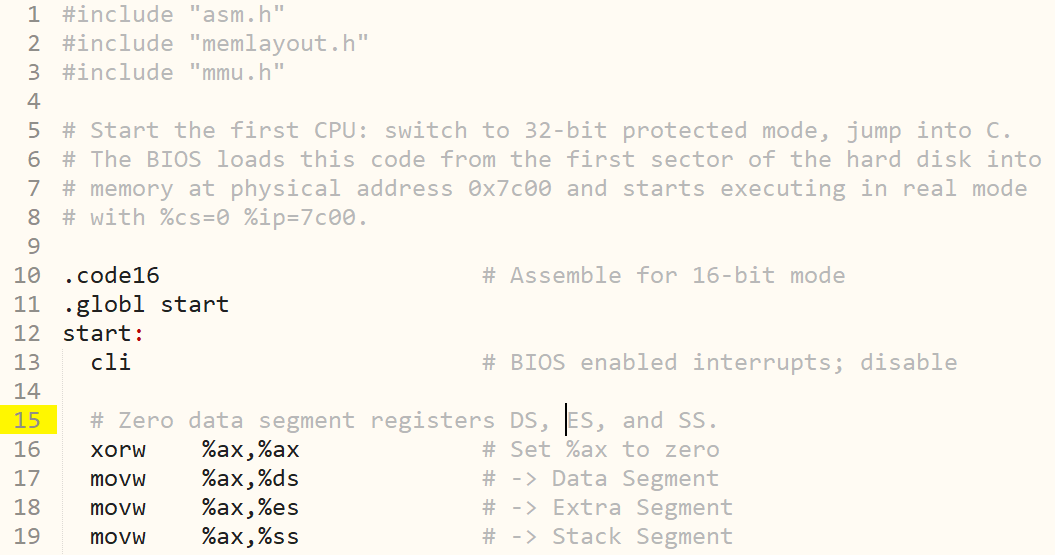
\includegraphics [width=1.0\textwidth]{figure//image89.png}
	%\caption{}\label{dianguang13}
\end{figure}

但是实模式刚运行完,很多遗留下的一些寄存器的值需要我整理下,所以我需要“在16~19行中 将 %ax 置零,然后把这个零值拷贝到三个段寄存器中, 将DS, ES, SS进行清零”。
实模式的东西处理完,我的重点是要转换到保护模式中去开始真正的工作。为此我需要打开A20开关, 将32位地址总线打开,使得地址位从20位切换到32位.
关于为什么需要打开A20开关,可以参考文档最后的附录部分.
下面的代码实现了打开A20开关.
\begin{figure}[H]
	\centering
	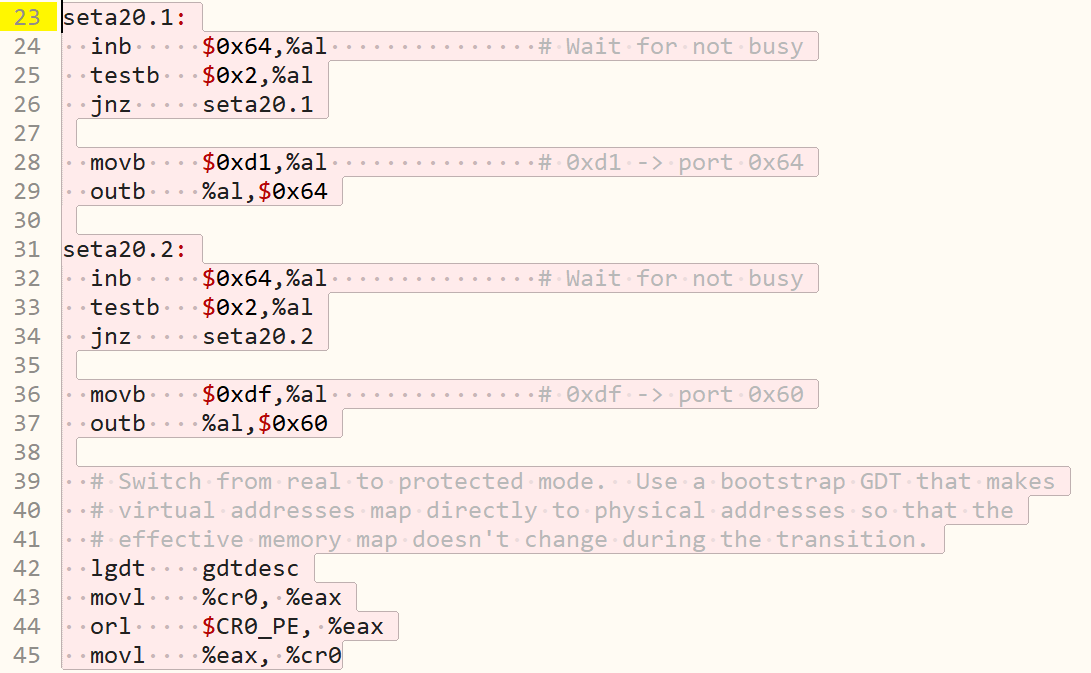
\includegraphics [width=1.0\textwidth]{figure//image90.png}
	%\caption{}\label{dianguang13}
\end{figure}
接下来加载全局符号表GDT
第42行代码通过引导加载器执行 lgdt指令来把指向 gdt 的指针 gdtdesc加载到全局描述符表(GDT)寄存器中。第44行正式开启保护模式(CR0\_PE=1)接下来第51行处理器还需要将16位模式(因为之前是实模式,所以目前还是处于16位的模式)切换到32位。由于我没法直接修改 \%cs,所以使用了一个 ljmp 指令ljmp \$(SEG\_KCODE<<3), \$start32。跳转指令会接着在下一行执行,但这样做实际上将 \%cs 指向了 gdt 中的一个代码描述符表项。该描述符描述了一个32位代码段,这样处理器就切换到了32位模式下。
\begin{figure}[H]
	\centering
	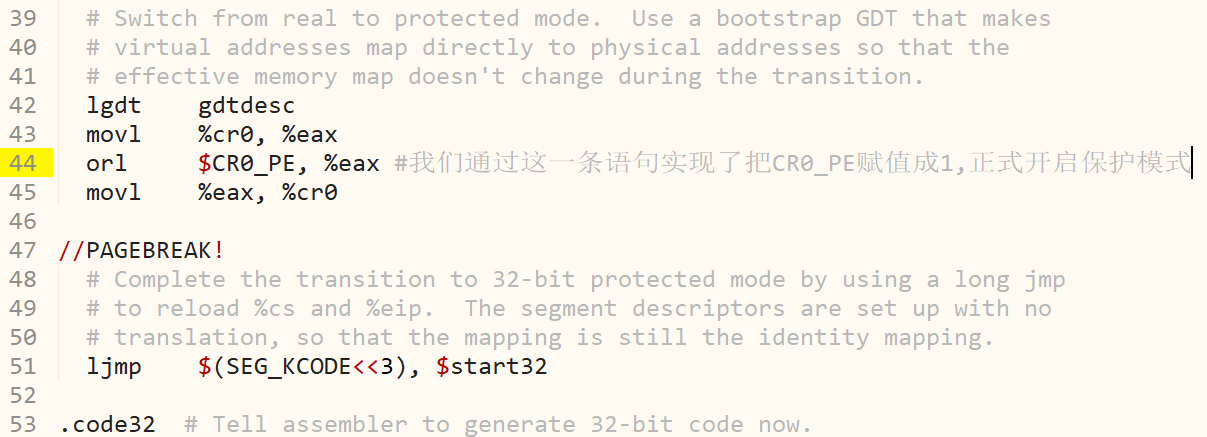
\includegraphics [width=1.0\textwidth]{figure//image91.png}
	%\caption{}\label{dianguang13}
\end{figure}

接下来完成保护模式之下的初始化数据,然后开始执行bootmain.c代码
\begin{figure}[H]
	\centering
	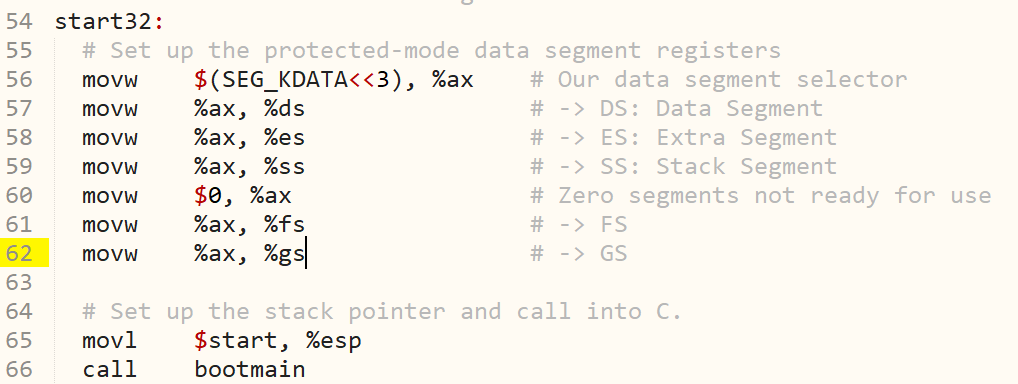
\includegraphics [width=1.0\textwidth]{figure//image92.png}
	%\caption{}\label{dianguang13}
\end{figure}


bootmain.c
在这个文件中主要有四个函数:bootmain、waitdisk、readsect和readseg。其中bootmain是加载内核,其余三个都是对磁盘进行访问的程序。
首先来看一下waitdisk、readsect和readseg。 readseg函数的作用是从磁盘的offset处开始读取count个字符到pa处。在读取数据时是通过调用readsect以扇区为单位进行的。因此在86行保证pa是从一个扇区起始位置开始,因此要对pa进行对齐。readsect是对磁盘进行读取,在读取之前每次调用waitdisk等待磁盘的准备过程,一旦磁盘准备好后就可以进行读取了。
\begin{figure}[H]
	\centering
	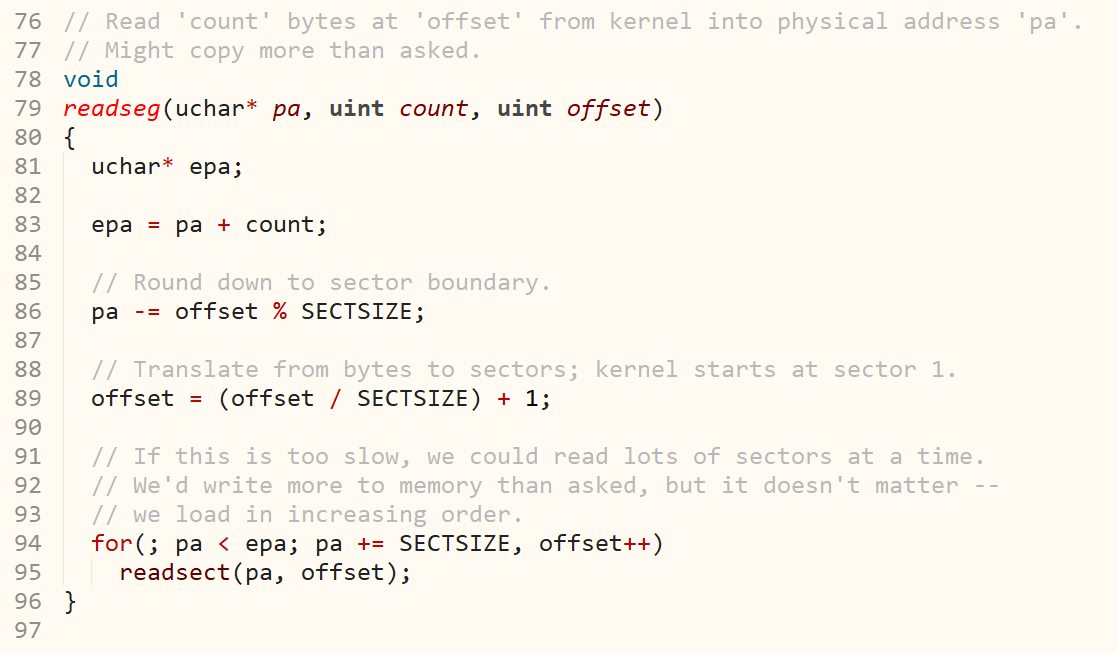
\includegraphics [width=1.0\textwidth]{figure//image93.png}
	%\caption{}\label{dianguang13}
\end{figure}



\begin{figure}[H]
	\centering
	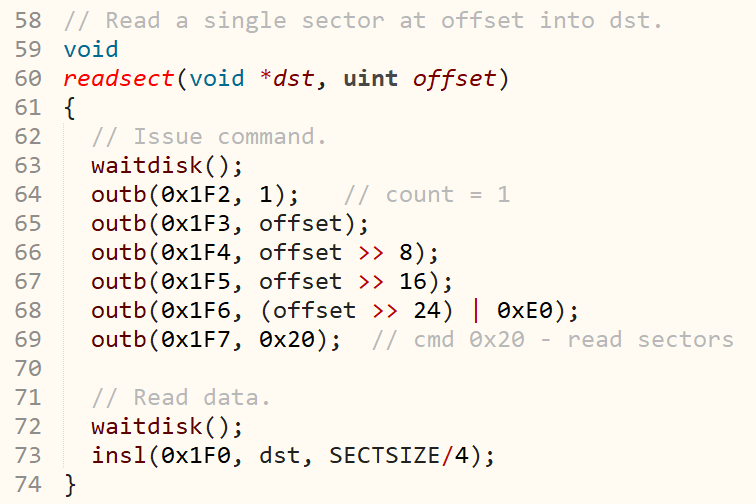
\includegraphics [width=1.0\textwidth]{figure//image94.png}
	%\caption{}\label{dianguang13}
\end{figure}
\begin{figure}[H]
	\centering
	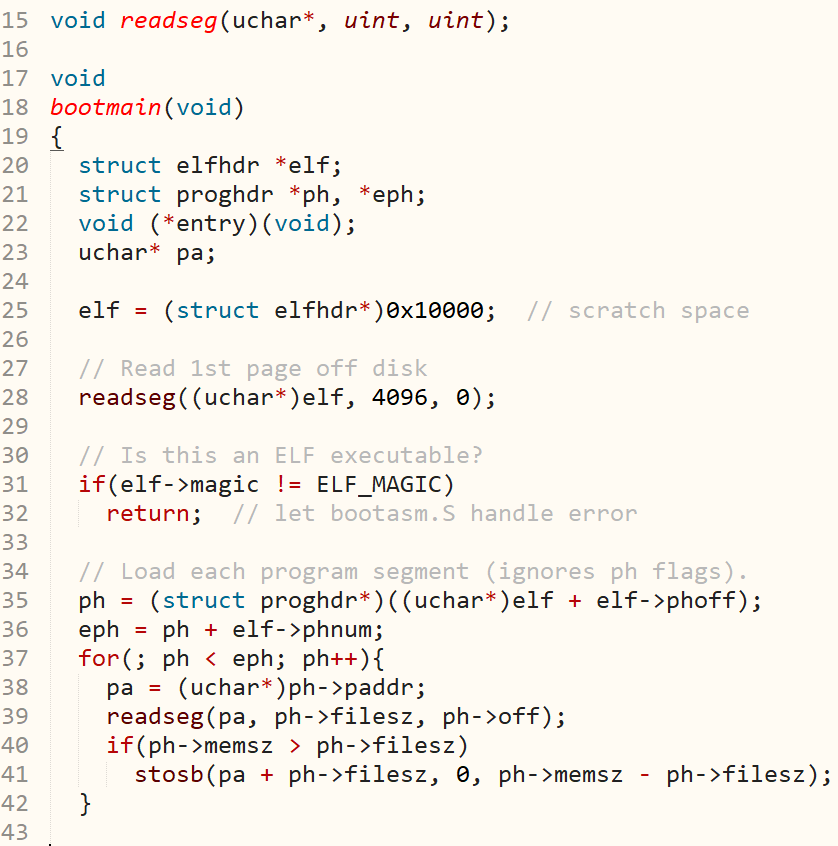
\includegraphics [width=1.0\textwidth]{figure//image95.png}
	%\caption{}\label{dianguang13}
\end{figure}
然后看一下bootmain过程。bootmain的目的是从磁盘中加载内核到内存中,其中内核是 ELF 格式的二进制文件。为了读取 ELF 头,在第28行bootmain 载入 ELF 文件的前4096字节,并将其拷贝到内存中 0x10000 处。其中包含了ELF执行文件格式的头。从中可以知道读取镜像的大小以及存放的位置
第31行通过 ELF 头检查这是否的确是一个 ELF 文件。
在第39行bootmain 调用 readseg 将数据从磁盘中载入,第41行并调用 stosb 将段的剩余部分置零。stosb使用 x86 指令 rep stosb 来初始化内存块中的每个字节。当完成拷贝后,在第46行bootmain获取内核入口程序的地址,然后进入该入口
bootloader紧接着就是entry开始运行,这个时候x86 的分页硬件在此时还没有开始工作;所以这时的虚拟地址是直接映射到物理地址上的。
boot loader 把 xv6 内核装载到物理地址 0x100000 处。之所以没有装载到内核指令和内核数据应该出现的 0x80100000,是因为小型机器上很可能没有这么大的物理内存。而之所以在 0x100000 而不是 0x0 则是因为地址 0xa0000 到 0x100000 是属于 I/O 设备的。
为了让内核的剩余部分能够运行,entry 的代码设置了页表,将 0x80000000开始的虚拟地址映射到物理地址 0x0 处。
它将 entrypgdir 的物理地址载入到控制寄存器 \%cr3 中。分页硬件必须知道 entrypgdir 的物理地址,因为此时它还不知道如何翻译虚拟地址;它也还没有页表。entrypgdir 这个符号指向内存的高地址处,但只要用宏 V2P\_WO减去 KERNBASE 便可以找到其物理地址。为了让分页硬件运行起来, xv6 会设置控制寄存器 \%cr0 中的标志位 CR0\_PG。

\begin{figure}[H]
	\centering
	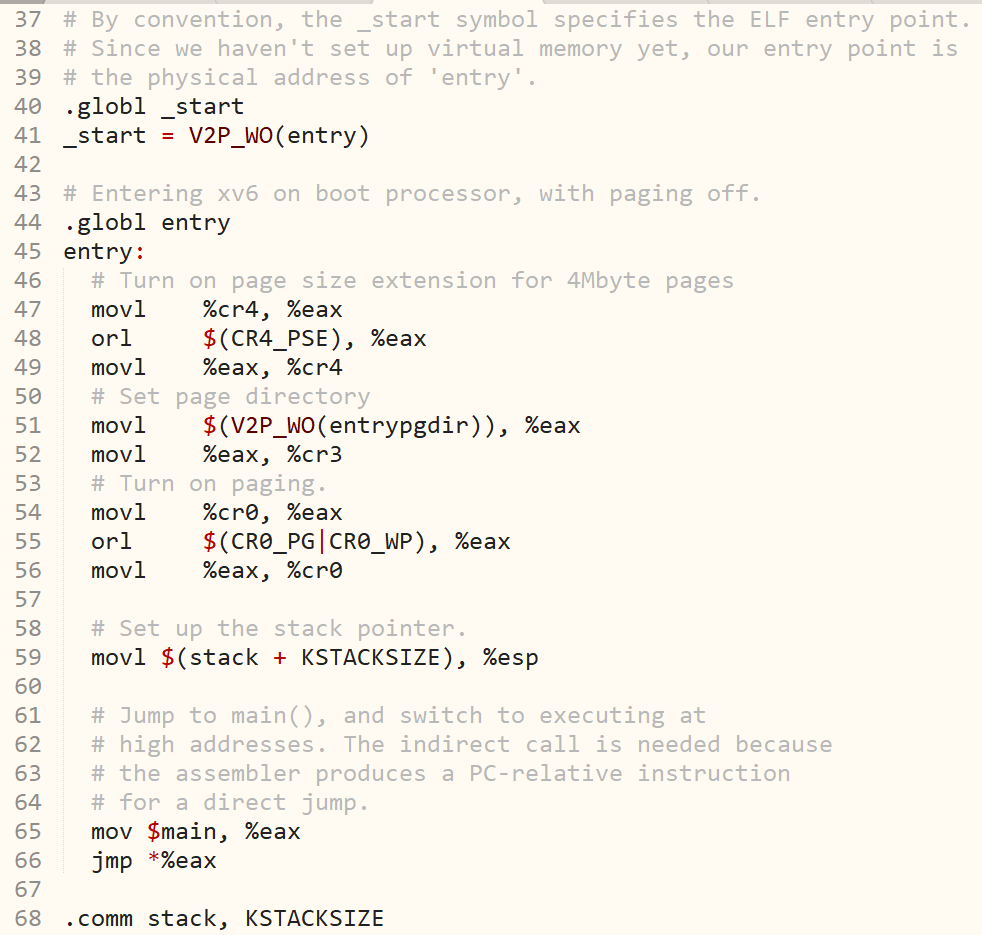
\includegraphics [width=1.0\textwidth]{figure//image96.png}
	%\caption{}\label{dianguang13}
\end{figure}
Entry 在完成设置页表和栈指针的操作之后,跳转到内核的 C 代码,并在内存的高地址中执行它了。
首先它将栈指针 \%esp 指向被用作栈的一段内存。所有的符号包括 stack 都在高地址,所以当低地址的映射被移除时,栈仍然是可用的。
entry 跳转到高地址的 main 代码中。我必须使用间接跳转,否则汇编器会生成 PC 相关的直接跳转(PC-relative direct jump),而该跳转会运行在内存低地址处的 main。 main 不会返回,因为栈上并没有返回 PC 值。好了,现在内核已经运行在高地址处的函数 main中了。

到现在为止,xv6的引导工作全部完成,接下来开始执行内核代码.
\section{xv6的进程与调度分析}






\subsection{进程的概念}
  程序与进程的概念是不可分的。当用户在计算机上运行一个程序时,此程序对应的进程就诞生了,并实际完成各种程序提供的功能,而用户关闭一个程序时,进程也随之终止。程序是为了完成某项任务编排的语句序列,它要告诉计算机如何执行,因此程序是需要通过CPU来运行的,且在程序的运行过程中需要占有计算机的各种资源(比如内存等)才能运行下去。如果计算机系统在任一时刻限制只有一个程序在运行,则程序在整个运行过程中独占计算机中的全部资源,这样整个程序运行和管理就简单了。就象在一个家中只住了一个人A,他想看书就到书房去看书,想睡觉就到睡房的床上去睡觉,想看电视就到电视厅看电视,想吃饭就去餐厅吃饭,没人和他抢占资源。但为了提高计算机系统的资源利用率,需要支持多个程序并发执行。这就会带来许多新的问题,如资源的共享与竞争,同步与互斥等。比如此人与B成家并有了小孩C,那就是三口之家同时住一套房,当A想去看足球比赛直播电视节目的时候,如果发现电视厅已经有B在坐着看连续剧电视节目了,A就得等待或干别的事情。除非A在买一个电视,并在另外一个房间看他的球比赛直播。由于程序是静态的,我看到的程序是存储在存储介质(如硬盘、光盘等)上的,它无法反映出程序执行过程中的动态特性,而且程序在执行过程中会不断申请资源或释放资源,这样让程序作为共享资源的基本单位是不合适的,所以需要引入一个概念,它能描述程序的执行过程而且可以作为共享资源的基本单位,这个概念就是进程。简单地说,一个进程是一个具有一定独立功能的程序在一个数据集合上的一次动态执行过程。每个进程都是整个应用的某一部分。操作系统在逻辑上维护了进程的运行状态信息,即与进程运行直接相关的CPU寄存器和栈空间(只有这样才能实现进程切换)。操作系统根据当前进程的情况设置进程的状态,并根据进程的状态(比如优先级)进行选择一个进程占用CPU并运行,这个过程成为调度。
进程的状态
进程从诞生到死亡要经历若干个阶段,也会有生老病死。简单地说,进程有三种状态:就绪、执行、等待。多种原因可以导致创建一个进程,比如,当操作系统把一个程序从硬盘调入内存后,在开始执行前,操作系统就要为此程序创建一个对应的进程。又比如,一个进程可以自己创建一个子进程,子进程被创建后就是在内存中,处于就绪态,所谓就绪态就是万事具备,只欠CPU这个东风了;一旦进程占有了CPU,就可以执行实际的工作了,其状态就变成了执行态;进程在执行中如果需要等待某个资源(如等硬盘输入数据),则进程会放弃CPU,且其状态就变为等待态,这时操作系统又会从处于就绪态的另一个进程中挑选一个进程占有CPU,则这另一个进程的状态就变成了执行态。当前一个进程所等到数据到来后,处于等待态的前一个进程又被唤醒,并把状态变成为就绪态。
在实际的操作系统中,进程的状态往往多于三种,比如找xv6中,进程具有多种状态,包括:EMBRO, SLEEPING, RUNNABLE, RUNNING和ZOMBIE。定义在proc.h文件中:
\begin{figure}[H]
	\centering
	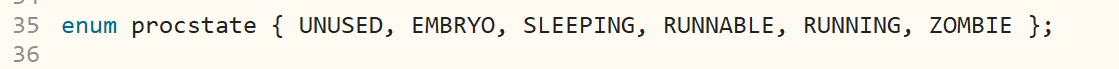
\includegraphics [width=1.0\textwidth]{figure//imageproc.png}
	%\caption{}\label{dianguang13}
\end{figure}

状态的含义如下:
\begin{itemize}
  \item 	UNUSED:进程未被创建(即进程控制块空闲)时的状态;
  \item 	EMBRYO:需要分配一个进程控制块且找到一个处于UNUSED状态的进程控制块时,把此进程控制块状态设置为要使用的状态;
  \item 	SLEEPING:进程由于等待某资源等原因无法执行,进入睡眠状态,即等待态;
  \item 	RUNNABLE:进程获得了除CPU之外的所有资源,处于可运行状态,即就绪态;
  \item 	RUNNING:进程获得CPU,正在运行的状态,即执行态;
  \item 	ZOMBIE:进程结束的状态
\end{itemize}
\subsection{进程控制块}
 程序的运行是通过进程体现的,操作系统对进程进行管理和控制,那么操作系统怎么了解到进程的状态并掌握进程占有的资源分配呢,而且进程做状态转换时CPU的现场保存在那呢?这实际是通过进程控制快(Process Control Block, 简称PCB)。PCB是进程 的唯一标志,在其中记录了进程的全部信息,相当于进程的档案。操作系统通过PCB感知进程的存在,通过PCB了解进程和控制 进程的运行。在xv6中,所有的CPU共享一个进程控制块池,即源代码中为proc.c中的proc(即进程控制块)数组。在这 个进程数组保存的进程控制块结构分成两类:一类是未使用的进程控制块结构,另一类是正在使用的进程控制块结构。每次要创建一个进程时,只需要从进程控制块数组中取得一个未使用进程控制块结构进行相应的处理即可。

xv6中结构体 struct proc包含进程大小、页表、内核栈、进程状态、进程id、父进程、目录等等,代码如下:
\begin{figure}[H]
	\centering
	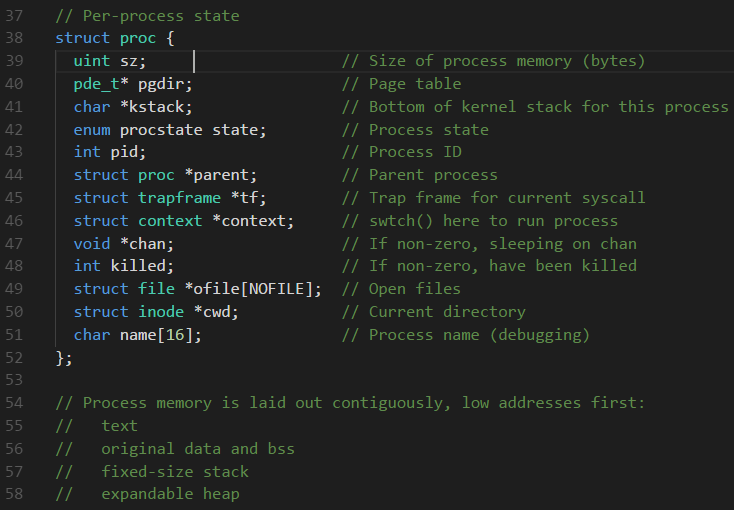
\includegraphics [width=1.0\textwidth]{figure//image97.png}
	%\caption{}\label{dianguang13}
\end{figure}

\begin{itemize}
  \item 	sz是记录进程所占有的内存空间大小;
  \item 	pgdir记录了进程页表的线性地址
  \item 	kstack是进程在内核态的栈;
  \item 	枚举类型变量 state记录了进程的状态;
  \item 	pid是进程的ID;
  \item 	parent记录父进程;
  \item 	tf是当前系统调用的中断帧;
  \item 	context是切换进程需要维护的硬件寄存器内容, 是进程运行的入口;
  \item 	chan不为NULL时,是进程睡眠时所挂的睡眠队列;
  \item 	killed不为0时,表示进程被杀死了;
  \item 	ofile数组是进程打开的文件数组;
  \item 	cwd是进程运行时所处的当前目录;
  \item 	name保存了进程的名字(用于调试)。

\end{itemize}
struct proc在proc.h中,并且在该文件之中定义了几个关键的数据结构。其中context是在内核进行上下文切换需要保存的寄存器: edi,esi,ebx,ebp,eip.
\begin{figure}[H]
	\centering
	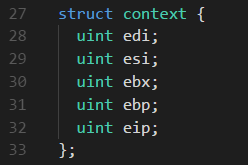
\includegraphics [width=1.0\textwidth]{figure//image98.png}
	%\caption{}\label{dianguang13}
\end{figure}


proc[NPROC]数组(在proc.c文件的12行)定义了xv6所能够支持的进程所需的相关数据,NPROC表示了xv6可支持进程个数。
\begin{figure}[H]
	\centering
	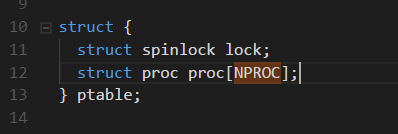
\includegraphics [width=1.0\textwidth]{figure//image99.png}
	%\caption{}\label{dianguang13}
\end{figure}



cpu结构是记录计算机中所有CPU的相关信息:

\begin{figure}[H]
	\centering
	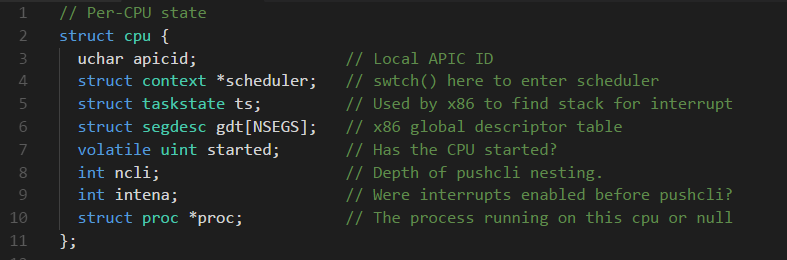
\includegraphics [width=1.0\textwidth]{figure//image100.png}
	%\caption{}\label{dianguang13}
\end{figure}

\begin{itemize}
  \item 	apicid 代表此CPU的id编号;
  \item 	scheduler表示scheduler的地址
  \item 	ts是Task state segment,用于在中断时找到栈
  \item 	gdt是此CPU的全局描述符表(GDT);
  \item 	started表示是否此CPU已经启动了;
  \item 	ncli表示执行pushcli函数的次数;
  \item 	intena表示是否能被打断;
  \item curproc是当前正在此CPU上运行的进程控制块;
\end{itemize}
spinlock的作用在于当进程请求得到一个正在被占用的锁时,将进程处于循环检查,等待锁被释放的状态。
\begin{figure}[H]
	\centering
	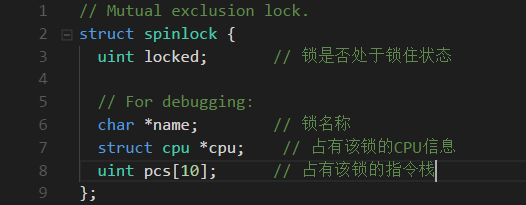
\includegraphics [width=1.0\textwidth]{figure//image101.png}
	%\caption{}\label{dianguang13}
\end{figure}

进程在虚拟内存中的布局如下:
\begin{figure}[H]
	\centering
	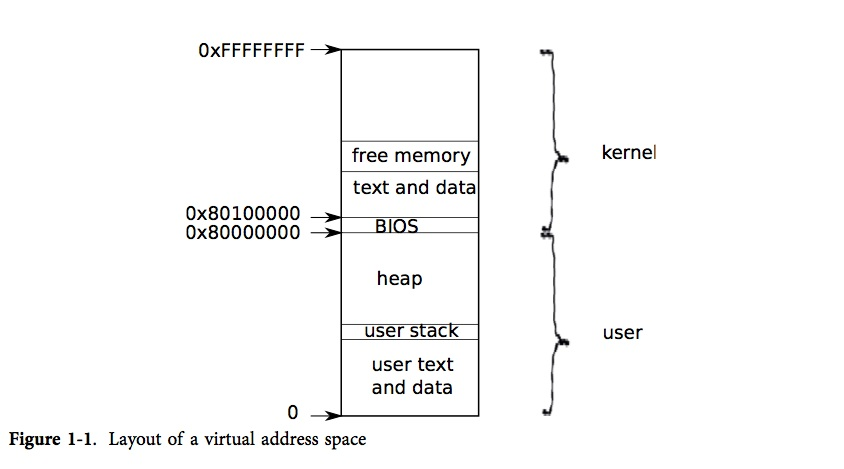
\includegraphics [width=1.0\textwidth]{figure//image102.png}
	%\caption{}\label{dianguang13}
\end{figure}
Xv6使用了一些全局变量来记录进程的状态.
进程数组 proc[NPROC]数组就是进程池。
进程池访问锁 proc\_table\_lock是一个spinlock是用来保护对进程池的临界区访问。
当前运行进程 curproc则是记录每个cpu当前运行的进程。
第一个进程 initproc是记录第一个创立的进程。这个进程十分特殊,它将托管所有没有父进程的进程(也就是父进程先于子进程结束)。
下一进程号 nextid是用来产生进程号的,在系统启动后会一直保持递增。
Xv6对于进程的处理过程
与进程相关的处理函数集中在proc.c中,下面将依次介绍相关处理过程。
进程管理初始化
pinit过程仅仅是初始化proc\_table\_lock锁。
\begin{figure}[H]
	\centering
	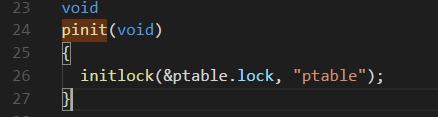
\includegraphics [width=1.0\textwidth]{figure//image103.png}
	%\caption{}\label{dianguang13}
\end{figure}

初始化用户进程init
userinit是初始化第一个用户进程init。其处理过程如下所示:
userinit 首先调用 allocproc。allocproc(第126行)的工作是在页表中分配一个槽(即结构体 struct proc),并初始化进程的状态,为其内核线程的运行做准备。
allocproc 会在 proc 的表中找到一个标记为 UNUSED的槽位。当它找到这样一个未被使用的槽位后,allocproc 将其状态设置为 EMBRYO,使其被标记为被使用的并给这个进程一个独有的 pid。接下来,它尝试为进程的内核线程分配内核栈。如果分配失败了,allocproc 会把这个槽位的状态恢复为 UNUSED 并返回0以标记失败。
\begin{figure}[H]
	\centering
	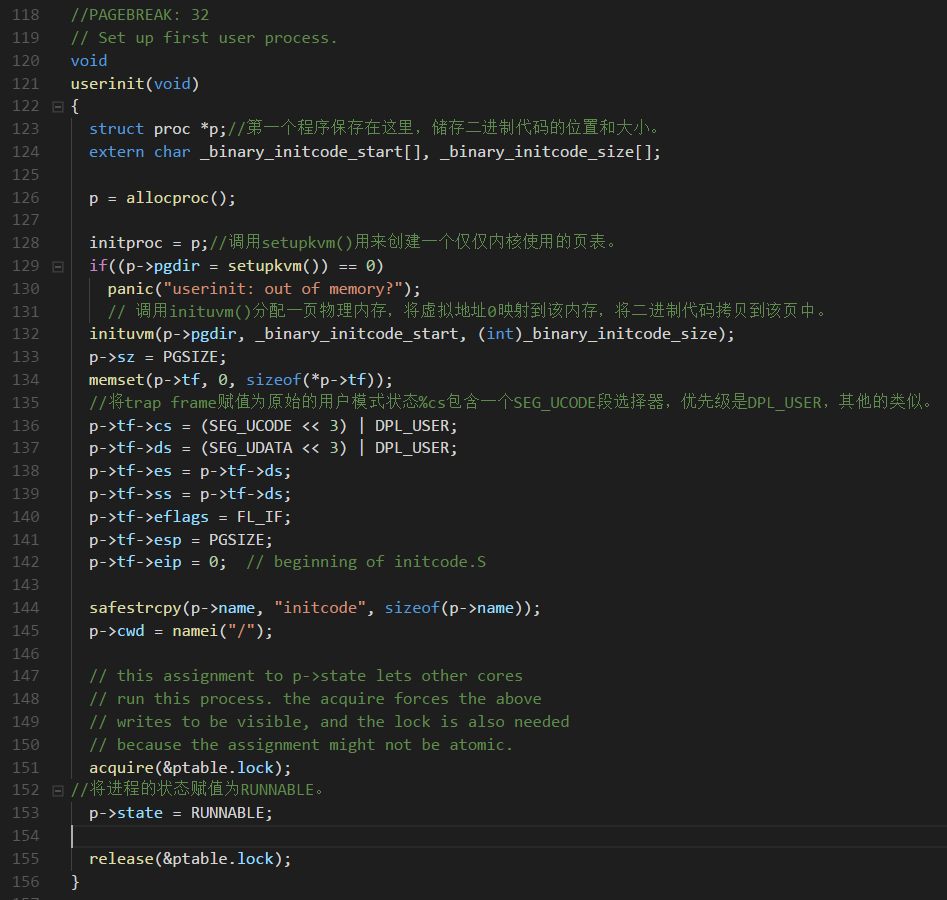
\includegraphics [width=1.0\textwidth]{figure//image104.png}
	%\caption{}\label{dianguang13}
\end{figure}


创建子进程
在xv6中,可以通fork来复制父进程内容并创建一个新的子进程。其处理过程如下所示:

一个进程调用 fork() 函数后,系统先给新的进程分配资源,例如存储数据和代码的空间。然后把原来的进程的所有值都复制到新的新进程中,只有少数值与原来的进程的值不同。相当于克隆了一个自己。fork() 函数通过系统调用创建一个与原来进程几乎完全相同的进程,也就是两个进程可以做完全相同的事(即复制了 fork() 函数后的代码),但如果初始参数或者传入的变量不同,两个进程也可以做不同的事。需要注意的是,两个进程拥有不同的内存空间和寄存器(fork()函数之前的变量值是一样的,但存储在不同地方),改变一个进程中的变量不会影响另一个进程。
fork()调用的一个奇妙之处就是它仅仅被调用一次,却能够返回两次,它可能有三种不同的返回值:
\begin{itemize}
  \item 在父进程中,fork() 返回新创建子进程的进程pid;
  \item 在子进程中,fork() 返回0;
  \item 如果出现错误,fork() 返回一个负值;
\end{itemize}



不同的进程有一个唯一的不同进程pid,通过 getpid() 函数可以知道当前进程pid,可以说我就是通过这个pid知道当前所在进程。
创建新进程成功后,系统中出现两个基本完全相同的进程,这两个进程执行没有固定的先后顺序,哪个进程先执行要看系统的进程调度策略。

调度进程
任何操作系统都可能碰到进程数多于处理器数的情况,这样就需要考虑如何分享处理器资源。理想的做法是让分享机制对进程透明。通常我对进程造成一个自己独占处理器的假象,然后让操作系统的 多路复用机制(multiplex) 将单独的一个物理处理器模拟为多个虚拟处理器。

记下来介绍 xv6 是如何调度进程.
Xv6系统允许有多个cpu,并且每一个cpu获取进程调度的权利是相同的。CPU在scheduler里面进行轮询操作,每次从线程池中选择一个RUNNABLE的进程进行运行。直到运行完毕,或一单位时间片结束,或者进程主动yield或sleep。
进程调度的时机:处于运行状态下的进程如果发生等待事件或者时间耗尽就会被xv6强制终止,变成就绪状态.这样的话,cpu就可以执行其他的进程,提高了cpu的使用率.

Xv6要完成进程切换的功能需要实现从运行中的一个进程切换到另一个进程并且让上下文切换透明化,还有就是xv6支持多个cpu,所以可能出现多个 CPU 同时切换进程的情况,那么我必须使用一个带锁的方案来避免竞争,最后还有进程退出时必须释放其占用内存与资源.

进程切换:当CPU启动之后,执行scheduler函数,无限循环。在每个周期里,从进程表中找到一个RUNNABLE的进程,切换为进程的上下文,此时开始执行函数。当函数运行结束时,调用return函数,此时切换为CPU的上下文,开始下一循环。

进程唤醒与睡眠:如果一个程序需要等待IO,则CPU会将其设置为睡眠状态,此时不能被执行。当IO信号到达时,执行的进程会将IO信号对应的进程设置为RUNNABLE,即唤醒。下一个scheduler周期的时候,该进程就可能会被执行,处理IO信号。

进程表锁:对于多处理器架构而言,需要用到进程表的时候都需要事先获得表的锁,当结束之后再释放,这样保证了对进程表操作的原子化,可以避免多处理器的竞争问题。


下面通过代码来具体介绍xv6如何实现进程调度部分.
scheduler对每个CPU进行进程调度。CPU到没有运行用户进程时,就会进入这个过程中。这个过程不停的从进程中选出一个RUNNABLE的进程,然后运行这个进程(通过swtch.S中的swtch函数进行)。


\begin{figure}[H]
	\centering
	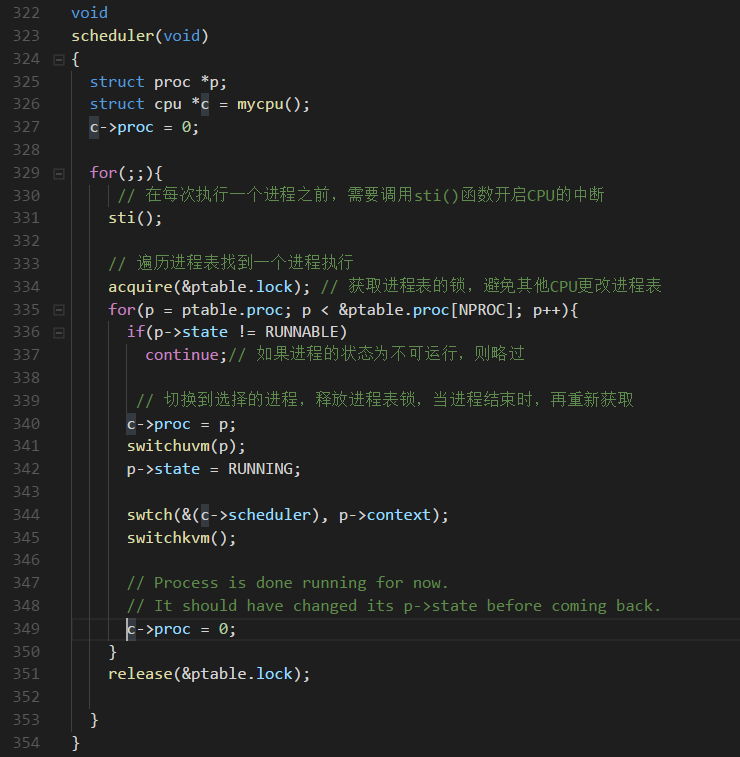
\includegraphics [width=1.0\textwidth]{figure//image105.png}
	%\caption{}\label{dianguang13}
\end{figure}


sched是放弃当前的用户进程,进入scheduler()。只需用通过swtch进行上下文切换即可。

\begin{figure}[H]
	\centering
	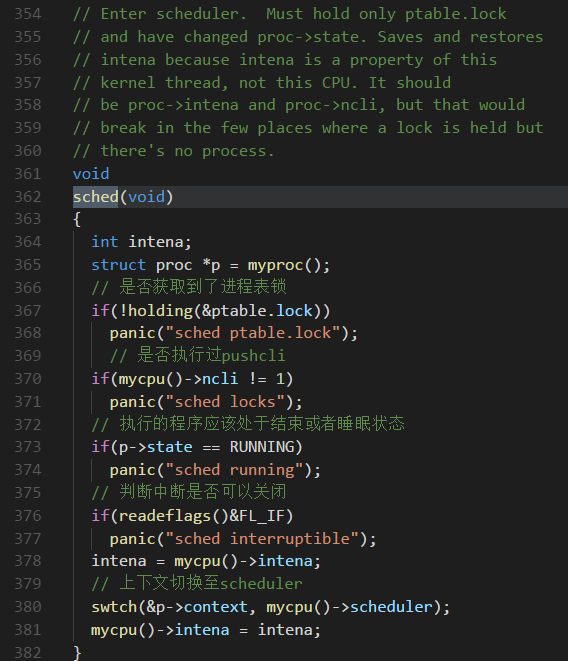
\includegraphics [width=1.0\textwidth]{figure//image106.png}
	%\caption{}\label{dianguang13}
\end{figure}
放弃CPU
yield是用户进程用来主动放弃当前CPU,进入scheduler()。因为进入scheduler需要加锁所以把proc\_table\_lock加上。
\begin{figure}[H]
	\centering
	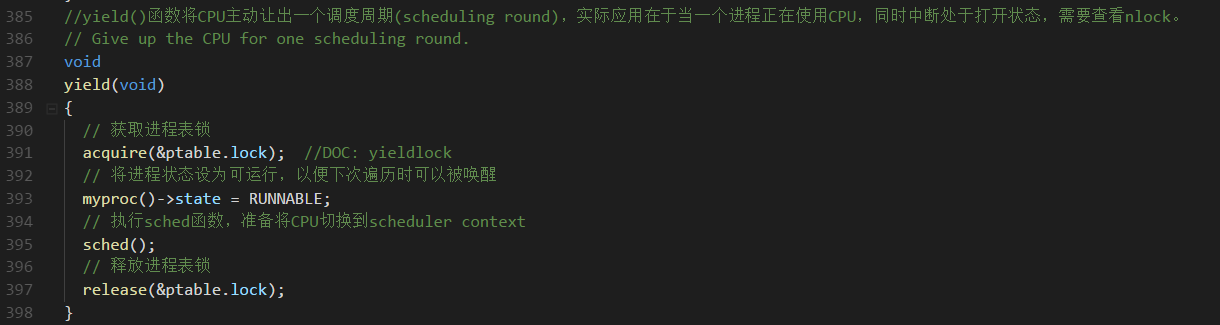
\includegraphics [width=1.0\textwidth]{figure//image107.png}
	%\caption{}\label{dianguang13}
\end{figure}


设置用户进程返回
forkret是用于新fork的进程进行返回地址用的。由于调用sys\_fork创建的新进程是通过shceduler()调用的,因此运行之前需要把proc\_table\_lock锁释放。
\begin{figure}[H]
	\centering
	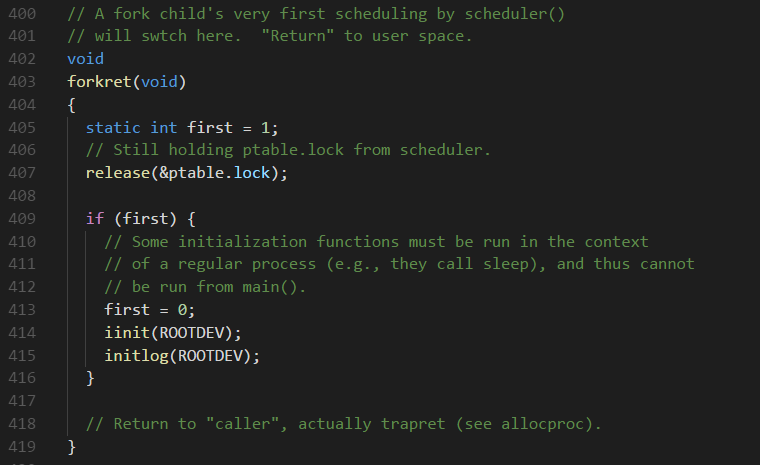
\includegraphics [width=1.0\textwidth]{figure//image108.png}
	%\caption{}\label{dianguang13}
\end{figure}

睡眠进程
sleep功能是让进程休眠。首先获得proc\_table\_lock,然后将记录chan,也就是说只有相关的chan才能把其唤起。然后调用sched()。当期被唤醒是,将继续运行,此时将chan等记录清空,并且将proc\_table\_lock锁释放,而获得lk锁。
\begin{figure}[H]
	\centering
	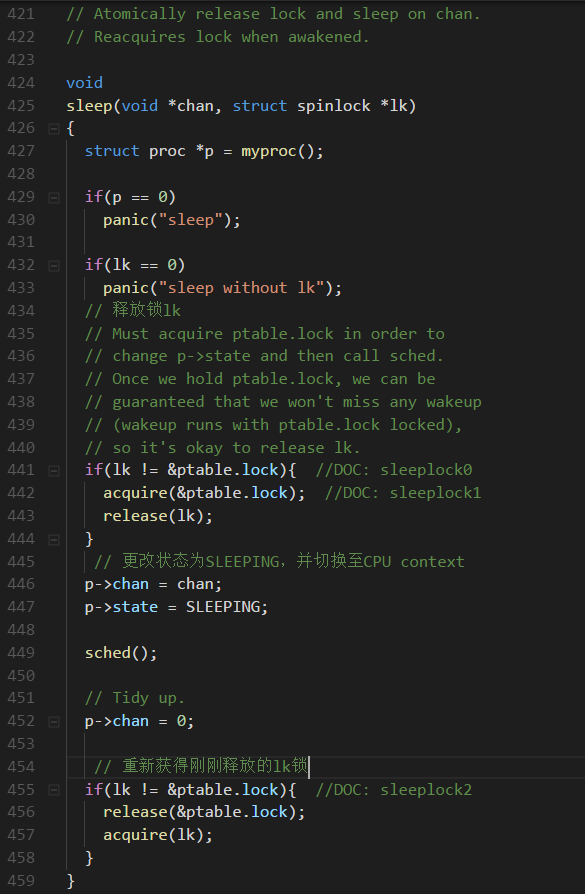
\includegraphics [width=1.0\textwidth]{figure//image109.png}
	%\caption{}\label{dianguang13}
\end{figure}


唤醒进程
值得注意的是,使进程进入睡眠需要两个锁,lk和ptable.lock,由于之前已经得到了ptable.lock,所以wakeup在此期间不会执行,直至进程完全进入睡眠状态,所以lk这个锁可以释放。
wakeup函数的主体部分位于wakeup1函数中。
wakeup功能是唤醒进程。先获取proc\_table\_lock,然后调用函数wakeup1,然后释放proc\_table\_lock。
wakeup1是将由于chan休眠的进程都唤醒,即把进程的状态由SLEEPING改成RUNNABLE。
\begin{figure}[H]
	\centering
	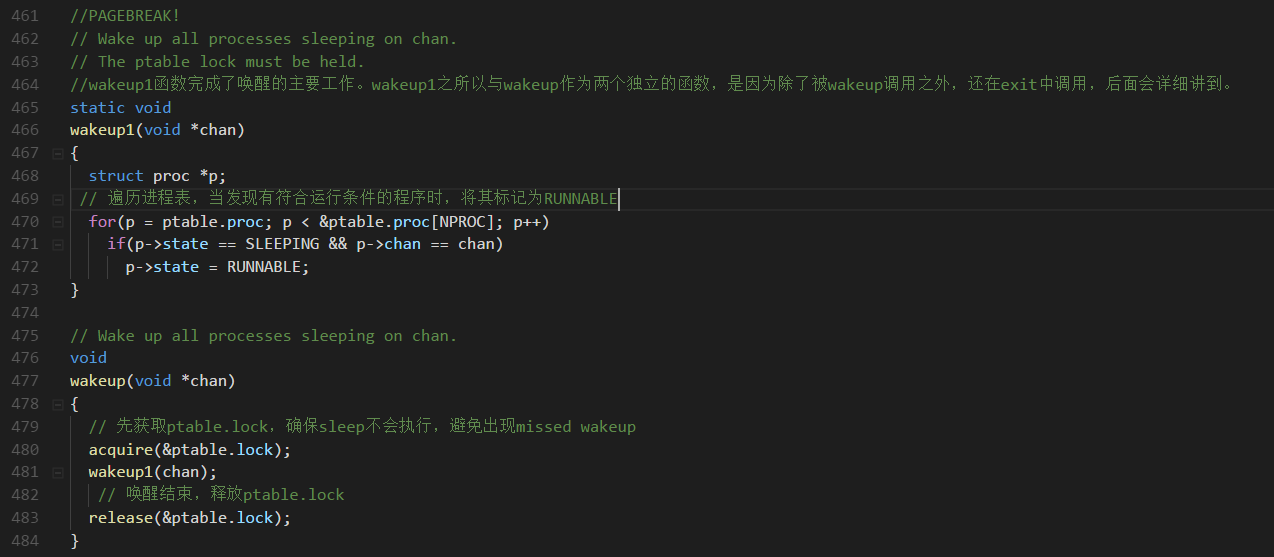
\includegraphics [width=1.0\textwidth]{figure//image110.png}
	%\caption{}\label{dianguang13}
\end{figure}

杀死进程
kill的作用是杀死某个进程。只需要从进程池中找到拥有相应进程ID的进程,将其killed状态置1即可。如果目标进程出于sleeping状态则将其设置成RUNNABLE使其尽早被杀掉。
详细的代码如下所示.
\begin{figure}[H]
	\centering
	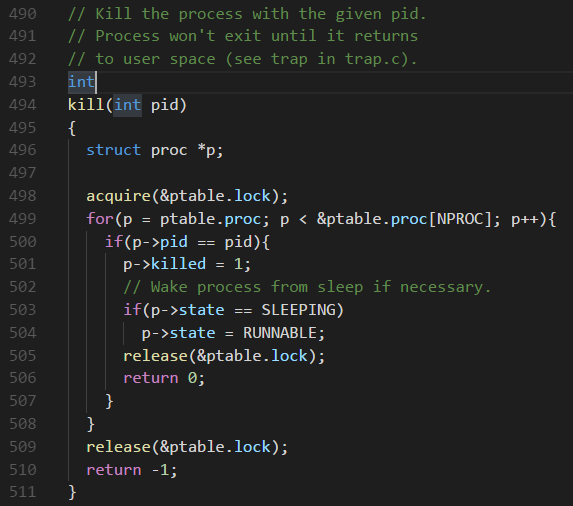
\includegraphics [width=1.0\textwidth]{figure//image111.png}
	%\caption{}\label{dianguang13}
\end{figure}
退出进程
exit完成了进程结束时的资源释放以及子进程处理等工作。在退出之前,用户进程需要关闭打开的文件(238-243行),将打开的文件夹关闭(358-359)。同时唤醒父进程,因为其可能出于wait状态。并将其子进程托管于init。然后改变其状态为ZOMBIE(等待父进程进行回收)。最后调用sched放弃CPU。
\begin{figure}[H]
	\centering
	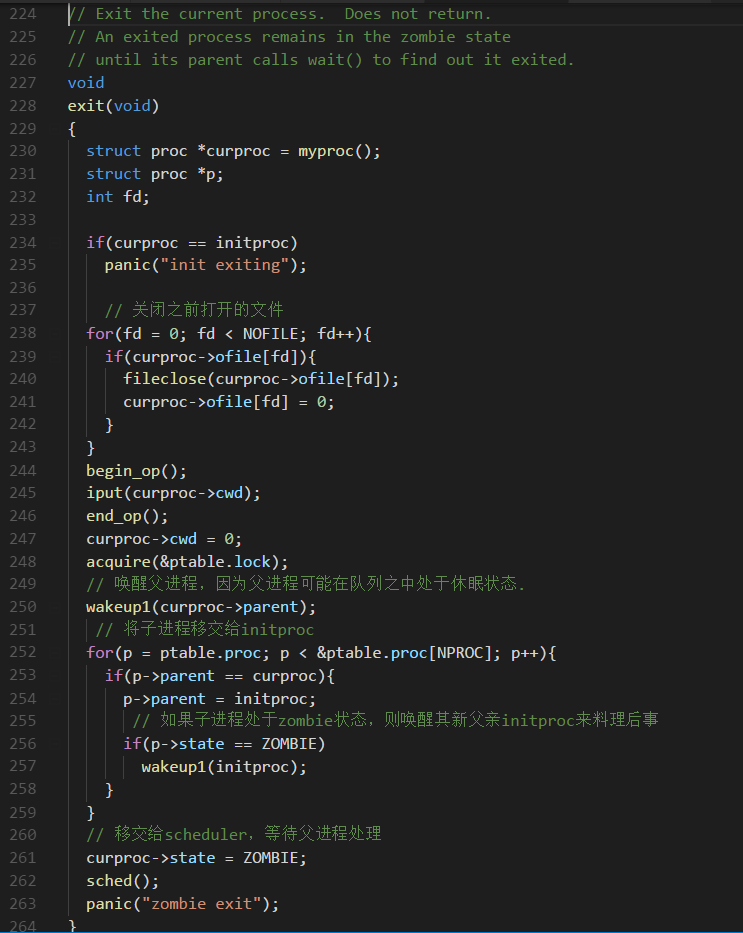
\includegraphics [width=1.0\textwidth]{figure//image112.png}
	%\caption{}\label{dianguang13}
\end{figure}

等待进程结束
wait是用于父进程等待子进程结束只用的。做法是不断的循环知道找到一个子进程变成ZOMBIE状态,则释放ZOMBIE子进程(回收其资源),然后结束循环返回其子进程的进程ID。在循环的时候需要判断是否被外部进程Kill,或有无活跃子进程,如果被杀死或无活跃子进程,则推出循环。
\begin{figure}[H]
	\centering
	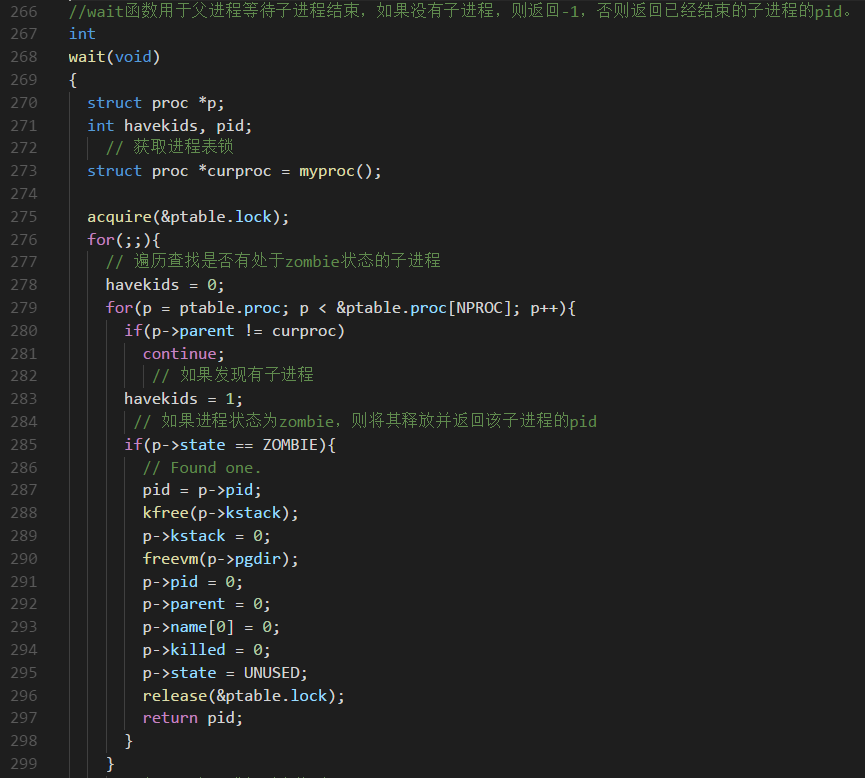
\includegraphics [width=1.0\textwidth]{figure//image113.png}
	%\caption{}\label{dianguang13}
\end{figure}


进程上下文切换
 在操作系统中通常也把上下文切换称为进程切换(process switch)。当操作系统决定运行另外的进程时,它需要保存当前正在运行进程的当前上下文(Context,也可称“运行状态信息”),即CPU寄存器中的全部内容。这些内容保存在进程的堆栈空间或特定的上下文保存区。完成保存工作后,操作系统就可以把下一个将要运行进程的当前上下文从该进程的栈或上下文保存区中恢复到CPU的寄存器中,这样就可以继续下一个进程的运行。这个过程叫做进程切换。一般有两种情况的上下文切换:
\begin{itemize}
  \item 	高优先级的进程因为需要某种临界资源,主动请求阻塞,让出处理器,此时将调度就绪状态的低优先级进程获得执行。这种切换称为进程级的上下文切换。
  \item 	进程因为时钟中断或其它中断到来而被打断,在中断服务例程处理完毕后,内核发现有更高优先级进程处于就绪态,则在中断处理结束后直接切换到高优先级进程执行。这种调度也称为中断级的上下文切换。
\end{itemize}



xv6 在低层次中实现了两种上下文切换:从进程的内核线程切换到当前 CPU 的调度器线程,从调度器线程
到进程的内核线程。xv6 永远不会直接从用户态进程切换到另一个用户态进程;这种切换是通过用户态-内核态切换(系统调用或中断)、切换到调度器、切换到新进程的内核线程、最后这个陷入返回实现的。

\begin{figure}[H]
	\centering
	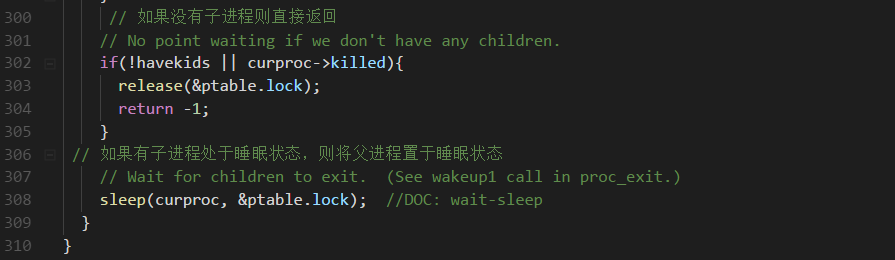
\includegraphics [width=1.0\textwidth]{figure//image114.png}
	%\caption{}\label{dianguang13}
\end{figure}



swtch.S
该文件主要执行上下文切换的功能.它并不了解线程,它只是简单地保存和恢复寄存器集合,即上下文信息。当进程让出 CPU 时,进程的内核线程调用 swtch来保存自己的上下文然后返回到调度器的上下文中。每个上下文都是以结构体 struct context* 表示的,这实际上是一个保存在内核栈中的指针。 swtch 有两个参数: struct context **old 、 struct context *new 。它将当前 CPU 的寄存器压入栈中并将栈指针保存在 *old 中。然后 swtch 将 new 拷贝到 \%esp 中,弹出之前保存的寄存器,然后返回。
下面是swtch.S的代码解释.
Swtch在第12和第13行从栈中弹出参数,放入寄存器 \%eax 和 \%edx中; swtch 必须在改变栈指针以及无法获得 \%esp 前完成这些事情。然后 swtch 在第18-21行压入寄存器,在当前栈上建立一个新的上下文结构。仅有被调用者保存的寄存器此时需要被保存;保存了旧寄存器后, swtch 就准备要恢复新的寄存器了。它将指向新上下文的指针放入栈指针中。新的栈结构和旧的栈相同,因为新的上下文其实是之前某次的切换中的旧上下文。所以 swtch 就能颠倒一下保存旧上下文的顺序来恢复新上下文。
\begin{figure}[H]
	\centering
	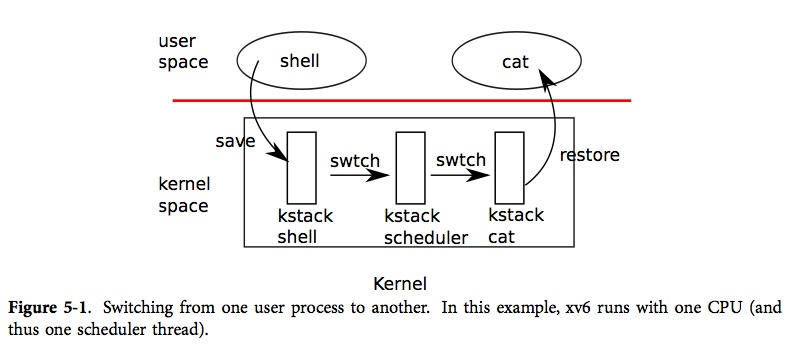
\includegraphics [width=1.0\textwidth]{figure//image115.png}
	%\caption{}\label{dianguang13}
\end{figure}


\section{xv6的内存管理}
内存管理机制是实时操作系统的重要组成部分。操作系统通过页表机制实现了对内存空间的控制。页表使得 xv6 能够让不同进程各自的地址空间映射到相同的物理内存上,还能够为不同进程的内存提供保护。 除此之外,我们还能够通过使用页表来间接地实现一些特殊功能。xv6 主要利用页表来区分多个地址空间,保护内存。另外,它也使用了一些简单的技巧,即把不同地址空间的多段内存映射到同一段物理内存(内核部分),在同一地址空间中多次映射同一段物理内存(用户部分的每一页都会映射到内核部分),以及通过一个没有映射的页保护用户栈。
下面我们就来详细介绍一下xv6的内存管理.
xv6初始化之后的物理内存图
\begin{figure}[H]
	\centering
	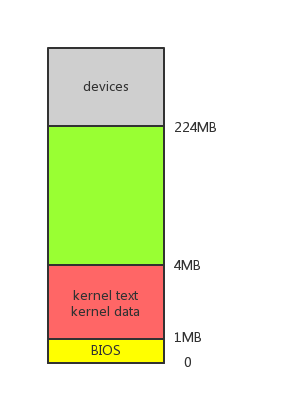
\includegraphics [width=1.0\textwidth]{figure//media//image1.png}
	%\caption{}\label{dianguang13}
\end{figure}
下面这个图展示的是XV6中虚拟地址到物理地址的映射关系.
\begin{figure}[H]
	\centering
	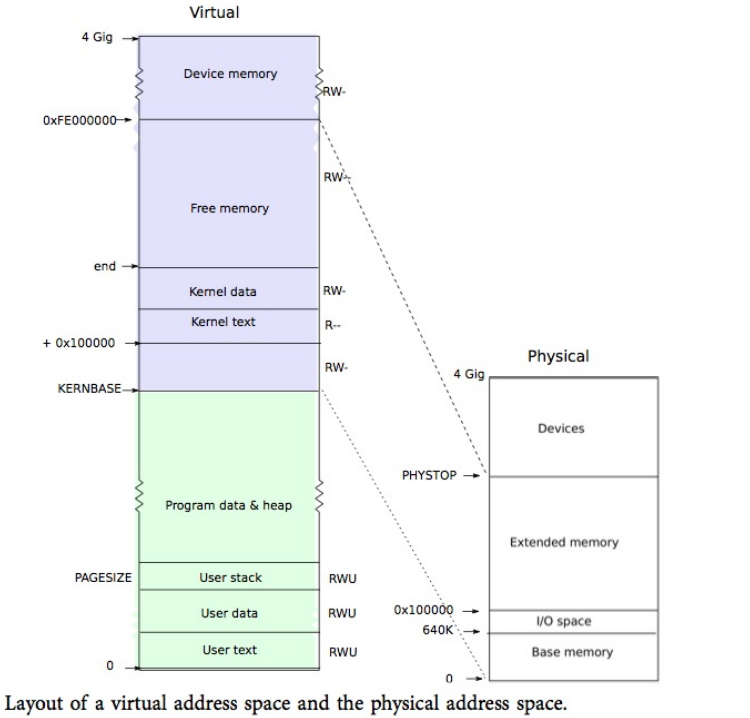
\includegraphics [width=1.0\textwidth]{figure//media//image2.png}
	%\caption{}\label{dianguang13}
\end{figure}

xv6 使用页表(由硬件实现)来为每个进程提供其独有的地址空间。页表将虚拟地址(x86 指令所使用的地址)翻译(或说“映射”)为物理地址(处理器芯片向主存发送的地址).
Xv6实现了两级页表,第一级页表有1024项(占有4096 字节),第二级页表也有1024项(占有4096 字节), xv6为每一个进程分配了这样的一个二级页表来实现将进程的虚拟地址转化为物理地址的过程. 分页硬件使用虚拟地址的高 10 位来决定对应页目录条目。如果想要的条目已经放在了页目录中,分页硬件就会继续使用接下来的 10 位来从页表页中选择出对应的 PTE。否则,分页硬件就会抛出错误。通常情况下,大部分虚拟地址不会进行映射,而这样的二级结构就使得页目录可以忽略那些没有任何映射的页表页。
在分页机制之中,虚拟地址的高20位来找到该虚拟地址在页表中的索引,然后把其高 20 位替换为对应 PTE 的 PPN。而低 12 位是会被分页硬件原样复制的。因此在虚拟地址-物理地址的翻译机制下,页表可以为操作系统提供对一块块大小为 4096(2\^{}12)字节的内存片,这样的一个内存片就是一页。
\begin{figure}[H]
	\centering
	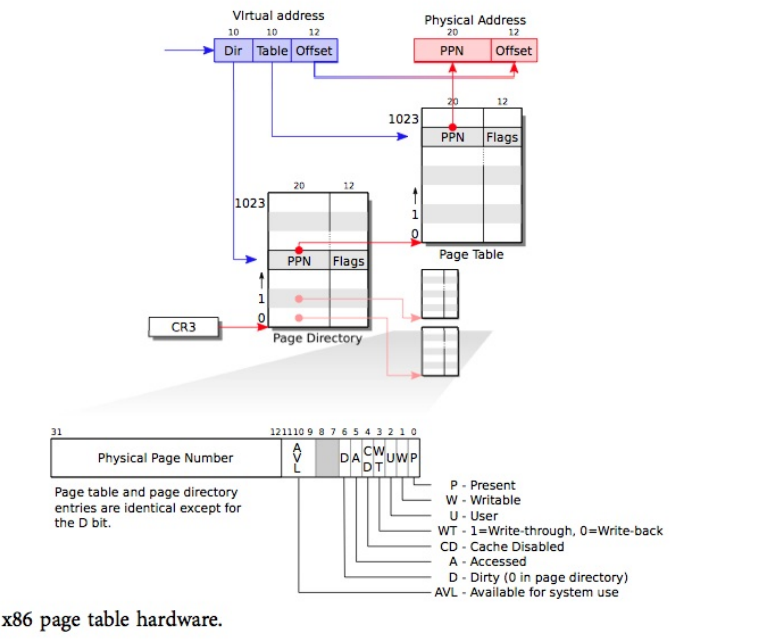
\includegraphics [width=1.0\textwidth]{figure//media//image3.png}
	%\caption{}\label{dianguang13}
\end{figure}

从图中可以看到,每个 PTE 都包含一些标志位,说明分页硬件对应的虚拟地址的使用权限。PTE\_P 表示 PTE 是否陈列在页表中:如果不是,那么一个对该页的引用会引发错误(也就是:不允许被使用)。PTE\_W 控制着能否对页执行写操作;如果不能,则只允许对其进行读操作和取指令。PTE\_U 控制着用户程序能否使用该页;如果不能,则只有内核能够使用该页。图 2-1 对此进行了说明。这些的标志位和页表硬件相关的结构体都在 mmu.h定义。
\begin{figure}[H]
	\centering
	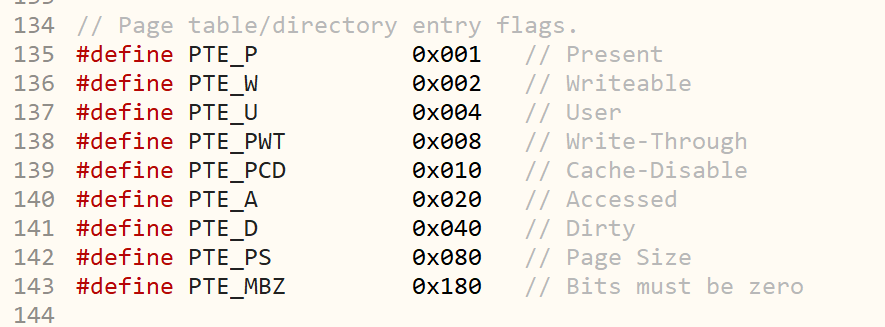
\includegraphics [width=1.0\textwidth]{figure//media//image4.png}
	%\caption{}\label{dianguang13}
\end{figure}

每个进程都有自己的页表,xv6 会在进程切换时通知分页硬件切换页表。如图所示,
\begin{figure}[H]
	\centering
	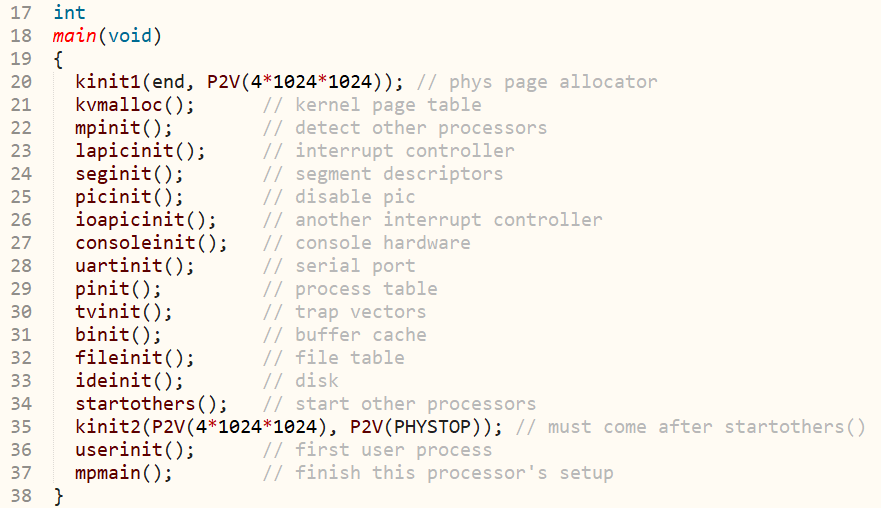
\includegraphics [width=1.0\textwidth]{figure//media//image5.png}
	%\caption{}\label{dianguang13}
\end{figure}

进程的用户内存从 0 开始,最多能够增长到 KERNBASE , 这使得一个进程最多只能使用 2GB 的内存。当进程向 xv6 要求更多的内存时,xv6 首先要找到空闲的物理页,然后把这些页对应的 PTE 加入该进程的页表中,并让 PTE 指向对应的物理页。xv6 设置了 PTE 中的 PTE\_U、 PTE\_W 、 PTE\_P 标志位。大多数进程是用不完整个内存空间的;xv6 会把没有被使用的 PTE 的 PTE\_P 标志位设为0。不同进程的页表将其用户内存映射到不同的物理内存中,因此每个进程就拥有了私有的用户内存。
xv6 在每个进程的页表中都包含了内核运行所需要的所有映射,而这些映射都出现在 KERNBASE 之上。它将虚拟地址KERNBASE:KERNBASE+PHYSTOP 映射到 0:PHYSTOP 。这样映射的原因之一是内核可以使用自己的指令和数据;原因之二是内核有时需要对物理页进行写操作,譬如在创建页表页的时候,而使得每一个物理页都在对应的虚拟地址上被映射就让这些操作变得很方便。这样的安排有一个缺点,即 xv6 无法使用超过 2GB 的物理内存。有一些使用内存映射的 I/O 设备的物理内存在0xFE000000 之上,对于这些设备 xv6 页表采用了直接映射。 KERNBASE 之上的页对应的 PTE 中, PTE\_U 位均被置 0,因而只有内核能够使用这些页。
每个进程的页表同时包括用户内存和内核内存的映射,这样当用户通过中断或者系统调用转入内核时就不需要进行页表的转换了。大多数情况下,内核都没有自己的页表,所以内核几乎都是在借用用户进程的页表。
Xv6如何建立一个地址空间
代码分析
在第21行main 调用 kvmalloc来创建并切换到一个拥有内核运行所需的 KERNBASE 以上映射的页表。
\begin{figure}[H]
	\centering
	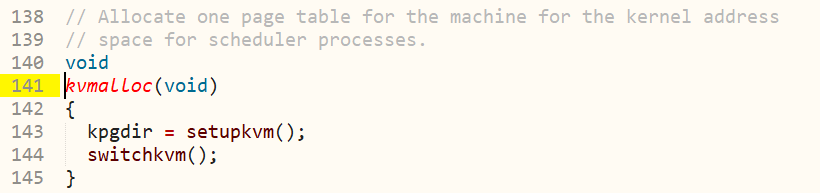
\includegraphics [width=1.0\textwidth]{figure//media//image6.png}
	%\caption{}\label{dianguang13}
\end{figure}

这里的大多数工作都是由 setupkvm完成的。
\begin{figure}[H]
	\centering
	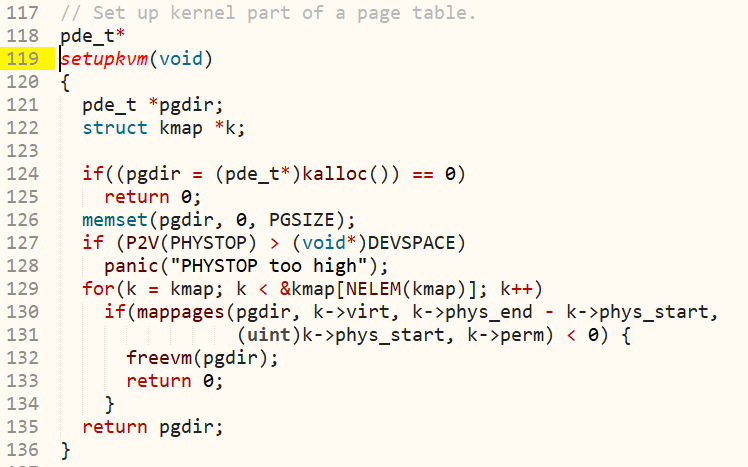
\includegraphics [width=1.0\textwidth]{figure//media//image7.png}
	%\caption{}\label{dianguang13}
\end{figure}
首先,它会分配一页内存来放置页目录,然后在第130行调用 mappages 来建立内核需要的映射,这些映射可以在 kmap数组中找到。这里的映射包括内核的指令和数据, PHYSTOP 以下的物理内存,以及 I/O 设备所占的内存。 setupkvm 不会建立任何用户内存的映射,这些映射稍后会建立。
\begin{figure}[H]
	\centering
	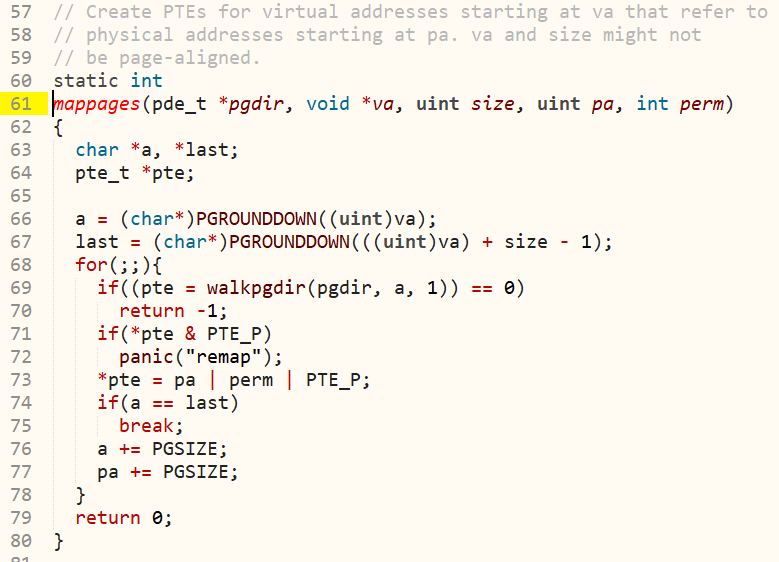
\includegraphics [width=1.0\textwidth]{figure//media//image8.png}
	%\caption{}\label{dianguang13}
\end{figure}
mappages做的工作是在页表中建立一段虚拟内存到一段物理内存的映射。它是在页的级别,即一页一页地建立映射的。对于每一个待映射虚拟地址, mappages 调用 walkpgdir 来找到该地址对应的 PTE 地址。然后初始化该 PTE 以保存对应物理页号、许可级别( PTE\_W 和/或 PTE\_U )以及 PTE\_P 位来标记该 PTE 是否有效.
\begin{figure}[H]
	\centering
	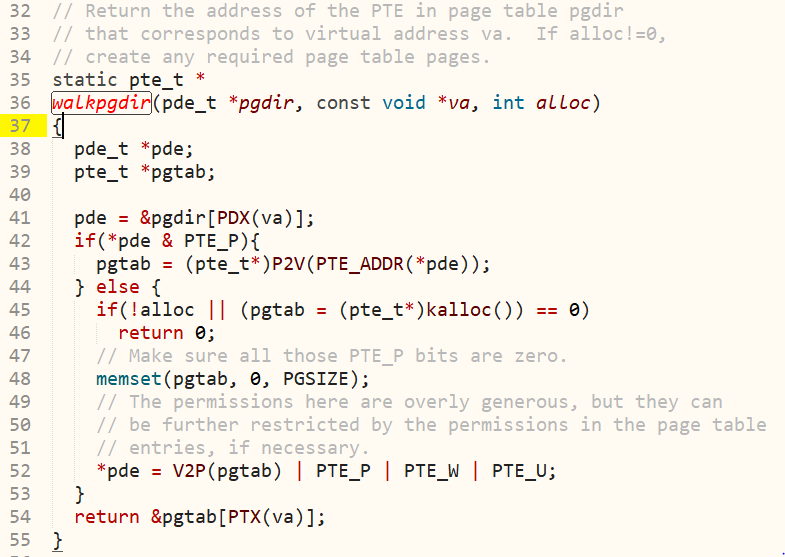
\includegraphics [width=1.0\textwidth]{figure//media//image9.png}
	%\caption{}\label{dianguang13}
\end{figure}
walkpgdir模仿 x86 的分页硬件为一个虚拟地址寻找 PTE 的过程。 walkpgdir 通过虚拟地址的前 10位来找到在页目录中的对应条目,如果该条目不存在,说明要找的页表页尚未分配;如果 alloc 参数被设置了, walkpgdir 会分配页表页并将其物理地址放到页目录中。最后用虚拟地址的接下来 10 位来找到其在页表中的 PTE 地址.
物理内存的分配
Xv6在运行时,内核需要为页表、进程的用户内存、内核栈及管道缓冲区分配空闲的物理内存。
xv6 使用从内核结尾到 PHYSTOP 之间的物理内存为运行时分配提供内存资源。每次分配,它会将整块 4096 字节大小的一页分配出去。xv6 还会通过维护一个物理页组成的链表来寻找空闲页。所以,分配内存需要将页移出该链表,而释放内存需要将页加入该链表。


\section{xv6的文件系统}
\begin{figure}[H]
	\centering
	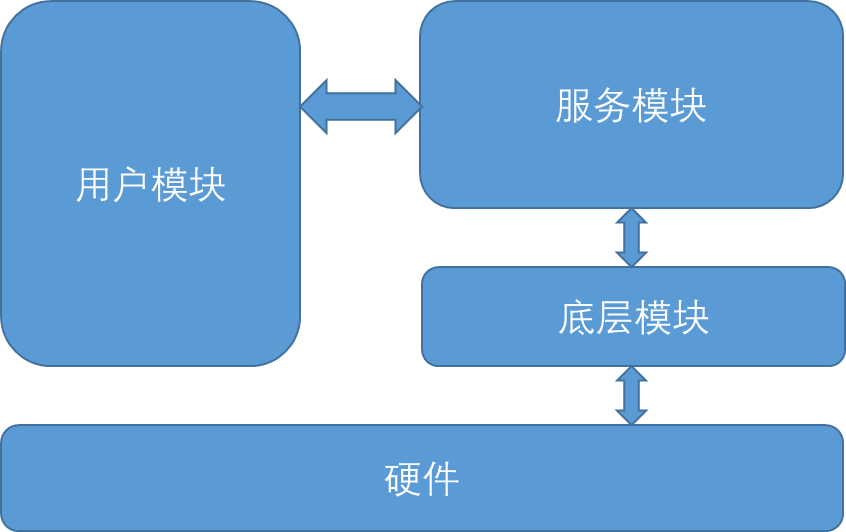
\includegraphics [width=1.0\textwidth]{figure//image147.png}
	%\caption{}\label{dianguang13}
\end{figure}

文件系统架构总体上分为3大模块,分别是用户模块,服务模块,底层模块。
服务器模块负责打包底层模块文件读写函数,为外界提供统一的文件读写接口。
底层模块负责详细的页面划分,加载,缓存以及控制磁盘驱动。
用户模块与文件服务系统进程通信来进行文件读写活动。
各层功能层次如下图

\begin{figure}[H]
	\centering
	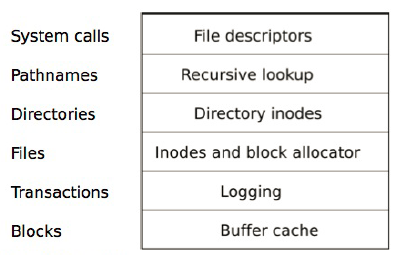
\includegraphics [width=1.0\textwidth]{figure//image148.png}
	%\caption{}\label{dianguang13}
\end{figure}

xv6 的文件系统分6层实现,如上图所示。最下面一层通过块缓冲读写 IDE 硬盘,它同步了对磁盘的访问,保证同时只有一个内核进程可以修改磁盘块。第二层使得更高层的接口可以将对磁盘的更新按会话打包,通过会话的方式来保证这些操作是原子操作(要么都被应用,要么都不被应用)。第三层提供无名文件,每一个这样的文件由一个 i 节点和一连串的数据块组成。第四层将目录实现为一种特殊的 i 节点,它的内容是一连串的目录项,每一个目录项包含一个文件名和对应的 i 节点。第五层提供了层次路经名(如/usr/rtm/xv6/fs.c这样的),这一层通过递归的方式来查询路径对应的文件。最后一层将许多UNIX 的资源(如管道,设备,文件等)抽象为文件系统的接口。



\subsection{	磁盘结构}

\begin{figure}[H]
	\centering
	\includegraphics [width=1.0\textwidth]{figure//image149.tmp}
	%\caption{}\label{dianguang13}
\end{figure}
磁盘扇区大小512字节,而xv6在此之上组织的块大小为4kB。Xv6是类UNIX操作系统,使用inode作为管理文件的基本单位,类似于jos实验中的文件元数据。
磁盘上文件结构是
\begin{itemize}
  \item 	Block0 引导扇区,分区表
  \item 	Block1 超级块
  \item 	Block2-k inodes块,存放磁盘文件的inode数据。
  \item 	Block k+1-t inodes块,Bitmap块,存储磁盘块占用信息
  \item 	Block t+1-l 数据块
  \item 	Block l+1-N-1 log块,存放日志信息。
\end{itemize}
\subsection{Inode结构}
\begin{figure}[H]
	\centering
	\includegraphics [width=1.0\textwidth]{figure//image150.tmp}
	%\caption{}\label{dianguang13}
\end{figure}
\begin{figure}[H]
	\centering
	\includegraphics [width=1.0\textwidth]{figure//imagefuck.png}
	%\caption{}\label{dianguang13}
\end{figure}
文件元数据使用inode结构体存储,包含文件名,文件大小,12个直接块,一个间接块。文件的前12个block号会存在直接块里,其他的block会存在间接块指向的block里,可以额外存储4096/4=1024个文件块。
此文件系统不支持双重间接块和三重间接块,所以文件不能大于1036个文件块。
\begin{figure}[H]
	\centering
	\includegraphics [width=1.0\textwidth]{figure//image151.png}
	%\caption{}\label{dianguang13}
\end{figure}

\subsection{	目录与普通文件}
文件系统以相同的方式管理目录文件与普通文件,以f\_type区分,当文件块描述目录时,关联数据块内容为目录下的其他文件File数据块。
\subsection{	块缓存}
\begin{figure}[H]
	\centering
	\includegraphics [width=1.0\textwidth]{figure//image152.png}
	%\caption{}\label{dianguang13}
\end{figure}
Xv6中我们通过缓存技术来实现访问磁盘块。该机制可以支持最大3GB的磁盘。
我们将文件系统服务进程的虚拟地址空间(0x10000000 (DISKMAP)到0xD0000000 (DISKMAP+DISKMAX))对应到磁盘的地址空间(3GB)。
由于现代磁盘大于3GB,在32位机器上的真正的文件系统实现会很麻烦。这种缓冲区高速缓存管理方法在64位地址空间的机器上仍然是合理的。
映射方法:我们假装整个磁盘都已经被缓存到内存中,当我们想访问虚拟空间中的一个页时,由于虚拟空间还没有被映射,会发生页错误。在页错误处理程序中则会实际进行磁盘块到虚拟地址的映射并将该块磁盘内容缓存到内存中。
此时就可以恢复文件系统进程进行正常的文件访问。
Bc\_pgfault函数负责处理页面错误,处理的同时进行页面映射并从磁盘中缓存对应的块到内存中。
处理的步骤:
\begin{itemize}
  \item 根据地址计算出对应的blockno(块编号)
  \item 检查地址范围是否超出(0x10000000 (DISKMAP)到0xD0000000 (DISKMAP+DISKMAX))的映射边界
  \item 检查块编号是否超出块数
  \item 将地址对齐到页起始位置
  \item 页面映射
  \item 调用ide\_read函数读取缓存块对应的数个磁盘页到内存中
  \item 更新脏位
\end{itemize}

\begin{figure}[H]
	\centering
	\includegraphics [width=1.0\textwidth]{figure//image1000.png}
	%\caption{}\label{dianguang13}
\end{figure}
\begin{figure}[H]
	\centering
	\includegraphics [width=1.0\textwidth]{figure//image1001.png}
	%\caption{}\label{dianguang13}
\end{figure}
Flush\_block函数负责将缓存中的块写回到磁盘中。
处理步骤:
\begin{itemize}
  \item 根据地址计算出对应的blockno(块编号)
  \item 检查地址范围是否超出(0x10000000 (DISKMAP)到0xD0000000 (DISKMAP+DISKMAX))的映射边界
  \item 检查如果对应块没有映射就不写回
  \item 检查如果对应块不是脏块(没有发生改动)就不写回
  \item  最后将缓存写回到磁盘,检查是否成功并更新脏位
\end{itemize}

\begin{figure}[H]
	\centering
	\includegraphics [width=1.0\textwidth]{figure//image1002.png}
	%\caption{}\label{dianguang13}
\end{figure}
\subsection{	磁盘ide驱动文件}
Fs/ide.c中实现了ide\_read 和 ide\_write方法
\begin{figure}[H]
	\centering
	\includegraphics [width=1.0\textwidth]{figure//image153.png}
	%\caption{}\label{dianguang13}
\end{figure}



\subsection{	文件操作}

fs / fs.c中提供了各种函数 来实现您将需要解释和管理File结构,扫描和管理目录文件的条目,从根目录文件系统来解析绝对路径名。有一下几个主要函数:
\begin{itemize}
  \item 	Walk\_path 完成目录解析
  \item 	File\_block\_walk 找到一个文件的某一块
  \item 	file\_get\_block 获取文件某一块
  \item 	file\_read 读取某一个文件
  \item 	file\_write 写入某一个文件
\end{itemize}
\subsection{	文件系统服务器}
与启动引导时把文件读写作为系统调用不同,而是作为一个用户进程于是我们在创建文件读写进程时需要把I/O读写权限打开
文件服务器进程采用轮询的方式接收用户进程发送的文件读写请求,向用户进程返回信息
\begin{figure}[H]
	\centering
	\includegraphics [width=1.0\textwidth]{figure//image154.png}
	%\caption{}\label{dianguang13}
\end{figure}


虚线下面的所有内容都是从常规环境到文件系统环境的读取请求的机制。从头开始,read(我们提供的)在任何文件描述符上工作,并简单地调度到适当的设备读取功能,在这种情况下 devfile\_read(我们可以有更多的设备类型,如管道)。 devfile\_read 实现read专门针对磁盘上的文件。这个和lib / file.c中的其他devfile\_*函数 实现了FS操作的客户端,并且都以大致相同的方式工作,将请求结构中的参数捆绑在一起,调用 发送IPC请求,解包并返回结果。该fsipc 函数只是处理向服务器发送请求和接收答复的常见细节。
文件系统服务器代码可以在fs / serv.c中找到。它在serve函数中循环,无休止地通过IPC接收请求,将该请求分派给相应的处理函数,并通过IPC发回结果。在读取的例子中, serve将调度到serve\_read,将处理特定的IPC细节读取请求,如解开请求结构,最后调用 file\_read实际执行文件读取。


\subsection{	用户使用的fd文件描述符}
\begin{figure}[H]
	\centering
	\includegraphics [width=1.0\textwidth]{figure//image155.png}
	%\caption{}\label{dianguang13}
\end{figure}



\subsection{		日志系统}


日志系统用来记录文件操作的记录,主要针对系统崩溃时可以使用日志来进行鉴别和恢复。
日志存在于磁盘末端已知的固定区域。它包含了一个起始块,紧接着一连串的数据块。起始块包含了一个扇区号的数组,每一个对应于日志中的数据块,起始块还包含了日志数据块的计数。xv6 在提交后修改日志的起始块,而不是之前,并且在将日志中的数据块都拷贝到文件系统之后将数据块计数清0。提交之后,清0之前的崩溃就会导致一个非0的计数值。
每一个系统调用都可能包含一个必须从头到尾原子完成的写操作序列,我们称这样的一个序列为一个会话,虽然他比数据库中的会话要简单得多。任何时候只能有一个进程在一个会话之中,其他进程必须等待当前会话中的进程结束。因此同一时刻日志最多只记录一次会话。
日志的操作:
\begin{lstlisting}
begin_trans();
bp = bread(...);
bp->data[...] = ...;
log_write(bp);
commit_trans();
begin_trans像锁一样,获取日志的控制权
bread操作缓冲块
log_write像是 bwrite
的一个代理,它把块中新的内容记录到日志中,并且把块的扇区号记录在内存。
commit_trans将日志的起始块写到磁盘上,类似于git的commit,
并产生一个检查点,可用于恢复。
\end{lstlisting}


\section{xv6 的I/O }
处理器必须像和主存交互一样同设备交互。x86 处理提供了特殊的 in, out 指令来在设备地址(称为'I/O 端口') 上读写。这两个指令的硬件实现本质上和读写内存是相同的。早期的 x86 处理器有一条附加的地址线:0表示从 I/O 端口读写,1则表示从主存读写。每个硬件设备会处理它所在 I/O 端口所接收到的读写操作。设备的端口使得软件可以配置设备,检查状态,使用设备;例如,软件可以通过对 I/O 端口的读写,使磁盘接口硬件对磁盘扇区进行读写。
很多计算机体系结构都没有单独的设备访问指令,取而代之的是让设备拥有固定的内存地址,然后通过内存读写实现设备读写。实际上现代 x86 体系结构就在大多数高速设备上(如网络、磁盘、显卡控制器)使用了该技术,叫做 内存映射 I/O。但由于向前兼容的原因, in, out 指令仍能使用,而比较老的设备如 xv6 中使用的 IDE 磁盘控制器仍使用这两个指令。
Xv6系统的I/O主要面向3个设备:磁盘,键盘,屏幕。
磁盘I/O控制方式为程序直接控制(查询)方式。调用磁盘ide驱动来进行硬件读写,向上提供统一的open,read,write等接口。
键盘输入方式为中断控制方式。将键盘中断捕获,交给控制台输入。
屏幕显示方式为程序直接控制(查询)方式。调用显示驱动向cga接口输出字符信息。
首先,我们从用户模式介绍xv6.
I/O 系统调用部分
\subsection{使用系统调用的文件描述符}
\begin{lstlisting}
read (int fd, char* buf, int len);
write (int fd, char* buf, int len);
stat (int fd, struct stat * );
dup (int fd);
close (int fd);

\end{lstlisting}

\subsection{命名服务}
\begin{lstlisting}
link (char ∗ oldpath , char ∗ newpath);
fd = open (char ∗ path , int flags);
unlink (char ∗ path);
mkdir (char ∗ path );
rmdir (char ∗ path );


\end{lstlisting}
还有管道函数用作文件缓冲
pipe (int pipefd[2]);
然后,我们开始进入xv6的核心
xv6核心是一个分层系统,其中文件层由pipe子系统和inode子系统组成,inode子系统包括name层、inode层、buffer层和driver层, 系统调用调用文件层,name层和inode层。
简单的介绍后,我们来探讨一下xv6如何在不同的硬件,结构和函数方法下,向用户模式提供统一的界面。
xv6 文件的抽象格式如下:
\begin{lstlisting}
struct file{
enum {FD_NONE, FD_PIPE , FD_INODE} type;
int ref; // reference count
char readable;
char writeable;
struct pipe∗ pipe;
struct inode ∗ ip;
uint off;
};
\end{lstlisting}
其中各个变量功能下文均有解释,并且均将细化到代码模块
\subsection{I/O 子系统}
由以下几个模块组成
FD\_PIPE.
FD\_INODE:
T\_FILE, T\_DIR, T\_DEV.
每个 I/O 子系统都是由一个结构体和一个操作集合来定义的,子系统中的各个模块将在下文予以解释
FD\_PIPE模块
\begin{lstlisting}
struct pipe{
struct spinlock lock;
char data[PIPESIZE];
uint nread;//读取的字符数目
uint nwrite;//写入的字符数目
intreadopen;//读取的文件仍然开启
intwriteopen;/写入的文件仍然开启
};

\end{lstlisting}
还有pipe的一些相关基本操作
pipalloc, pipeclose, piperead, pipewrite.
FD\_INODE模块
\begin{lstlisting}
struct inode{
uint dev;//设备数字
uint inum;//Inode数字
int ref;//Reference count
int flags;//IBUSY,IVALID
short type;// inode的磁盘镜像
short major;
short minor;
short nlink;
uint size;
uint addrs[NDIRECT+1];
};


\end{lstlisting}
F\_INODE相关方法
Listing1:读入T\_FILE or T\_DIR
调用如下方法
namei, create, ilock, readi, writei, stati, iunlock, iput
Listing2:读入T\_DEV
consoleread, consolewrite
\subsection{文件层的系统调用}
sys dup, sys read, sys write, sys fstat, sys close.

在fd系统调用中使用的函数
\begin{lstlisting}
struct file ∗ filedup(struct file ∗f)
fileclose(struct file ∗f);
fileread(struct file ∗f, char ∗buf, int len);
filewrite(struct file ∗f,char∗ buf, int len);
filestat(struct file∗f, struct stat∗s);



\end{lstlisting}
fdalloc:用于返回最低限度的被数字标记的空余文件槽.
\begin{lstlisting}
static int fdalloc(struct file ∗f){
    int fd;
    for(fd = 0;fd < NOFILE; fd ++){
        if(proc−>ofile[fd]==0){
            proc−>ofile[fd] = f;
            return fd;
        }
    }
    return −1;
}

\end{lstlisting}
sys\_dup部分
\begin{lstlisting}
sys_dup(void){
struct file ∗f;
int fd;
if(argfd(0,0,&f)<0) return −1;
if((fd = fdalloc(f))<0) return −1;
filedup(f);
return fd;
}

\end{lstlisting}
sys\_read部分
\begin{lstlisting}
int sys_read(void){
struct file ∗f;
int n;
char ∗p;
if(argfd(0,0,&f)<0||argint(2,&n)<0||argptr(1,&p,n)<0) return −1;
return fileread(f,p,n);
}

\end{lstlisting}

sys\_write部分
\begin{lstlisting}
int sys_write(void){
struct file ∗f;
int n;
char ∗p;
if(argfd(0,0,&f)<0||argint(2,&n)<0||argptr(1,&p,n)<0) return −1;
return filewrite(f,p,n);
}

\end{lstlisting}
sys\_fstat部分
\begin{lstlisting}
int sys_fstat(void){
struct file ∗f;
struct stat ∗st;
if(argfd(0,0,&f)<0||argptr(1,(void∗)&st,sizeof(∗st))<0) return−1;
return filestat(f,st);
}
\end{lstlisting}
sys\_close部分
\begin{lstlisting}
int sys_close(void){
int fd;
struct file∗f;
if(argfd(0,&fd,&f)<0) return −1;
proc−>ofile[fd]=0;
fileclose(f);
return 0;
}
\end{lstlisting}

文件层的实现通过以下五个函数:
filedup,fileread,filewrite,filestat,fileclose.
我们先来看一下ofile/file/inode/pipe 的执行流程
\subsection{ 无文件开启时}
\begin{figure}[H]
	\centering
	\includegraphics [width=1.0\textwidth]{figure//image156.png}
	%\caption{}\label{dianguang13}
\end{figure}

\subsection{ 执行open(”/carmi/f0”)}
\begin{figure}[H]
	\centering
	\includegraphics [width=1.0\textwidth]{figure//image157.png}
	%\caption{}\label{dianguang13}
\end{figure}
\begin{figure}[H]
	\centering
	\includegraphics [width=1.0\textwidth]{figure//image158.png}
	%\caption{}\label{dianguang13}
\end{figure}
\subsection{ 执行dup(0)}	
\begin{figure}[H]
	\centering
	\includegraphics [width=1.0\textwidth]{figure//image159.png}
	%\caption{}\label{dianguang13}
\end{figure}
\subsection{ 执行close(0)}	
\begin{figure}[H]
	\centering
	\includegraphics [width=1.0\textwidth]{figure//image160.png}
	%\caption{}\label{dianguang13}
\end{figure}
\subsection{ 	执行dup(1)}
\begin{figure}[H]
	\centering
	\includegraphics [width=1.0\textwidth]{figure//image161.png}
	%\caption{}\label{dianguang13}
\end{figure}
\subsection{ 	执行open(”/console”)}
\begin{figure}[H]
	\centering
	\includegraphics [width=1.0\textwidth]{figure//image162.png}
	%\caption{}\label{dianguang13}
\end{figure}
\subsection{ 	执行fork()}
\begin{figure}[H]
	\centering
	\includegraphics [width=1.0\textwidth]{figure//image163.png}
	%\caption{}\label{dianguang13}
\end{figure}


\subsection{ 	执行P0 close(1)}
\begin{figure}[H]
	\centering
	\includegraphics [width=1.0\textwidth]{figure//image164.png}
	%\caption{}\label{dianguang13}
\end{figure}
\subsection{ 	执行P1 close(2)}
\begin{figure}[H]
	\centering
	\includegraphics [width=1.0\textwidth]{figure//image165.png}
	%\caption{}\label{dianguang13}
\end{figure}
\subsection{ 	执行P0 pipe()}
\begin{figure}[H]
	\centering
	\includegraphics [width=1.0\textwidth]{figure//image166.png}
	%\caption{}\label{dianguang13}
\end{figure}

\subsection{文件层调度}

文件层将调度一下子系统之一:
\begin{itemize}
  \item pipe.
 \item inode.
\end{itemize}

pipe子系统和inode层使用的函数
Pipe子系统:
\begin{itemize}
  \item piperead(pipe *p, char *addr, int len);
 \item pipewrite(pipe *p ,char *addr, int len);
 \item pipeclose(pipe *p ,int writeside);
\end{itemize}

inode子系统:
\begin{itemize}
  \item ilock(inode *ip);
  \item iunlock(inode *ip);
 \item readi(inode *ip, char *adr, int len);
 \item writei(inode *ip, char* adr, int len);
 \item iput(inode *ip);
 \item stati(inode *ip, stat* stat);
 \item begintrans();
 \item committrans();
\end{itemize}




模块详细说明
file\_dup模块
\begin{lstlisting}
struct file∗ file_dup(struct file∗f){
acquire(&ftable.lock);
if(f−>ref<1) panic(”filedup”);
f−>ref++;
release(&ftable.lock);
return f;
}
\end{lstlisting}

根据类型,file\_read将读取委托给以下其中一个:
管道,readi。
对于FD\_INODE类型,处理文件位置。
file\_read模块
\begin{lstlisting}
int file_read(structfile ∗f, char ∗addr,int n){
int r;
if(f−>readable==0) return −1;
if(f−>type==FDPIPE) return pipe_read(f−>pipe,addr,n);
if(f−>type==FDINODE){
ilock(f−>ip);
if((r=readi(f−>ip,addr,f−>off,n))>0) f−>off+=r;
iunlock(f−>ip);
return r;
}
panic(”fileread”);
}
\end{lstlisting}
根据类型,filewrite将写入委托给以下其中一个:
pipe写入,writei。
对于FD\_INODE类型,处理文件位置。
file\_write模块
\begin{lstlisting}
int file_write(struct file ∗f, char∗ addr, int n){
if(f−>writable==0) return−1;
if(f−>type==FDPIPE) return pipe_write(f−>pipe,addr,n);
if(f−>type==FDINODE){
int max=((LOGSIZE−1−1−2)/2)∗512;
for(int i=0;i<n;){
int n1=n−i;
if(n1>max) n1=max;
begintrans();
ilock(f−>ip);
if((r=writei(f−>ip,addr+i,f−>off,n1))>0) f−>off+=r;
iunlock(f−>ip);
committrans();
if(r<0) break;
if(r!=n1) panic(”shortfilewrite”);
i+=r;
}
return i==n ? n:−1;
}
panic(”filewrite”);
}
\end{lstlisting}
reference count已更新。
如果reference count下降到零,我们委托给其中一个:
pipe关闭, iput。
由于iput我们必须释放需要注意,因此需要
复制文件结构。
file\_stat模块
\begin{lstlisting}
int file_stat(structfile ∗f,structstat ∗st){
if(f−>type==FDINODE){
ilock(f−>ip);
stati(f−>ip,st);
iunlock(f−>ip);
return 0;
}
return −1;
}
\end{lstlisting}
file\_close模块
\begin{lstlisting}
void file_close(struct file ∗f){
acquire(&ftable.lock);
if(f−>ref<1) panic(”fileclose”);
if(−−f−>ref>0){
release(&ftable.lock);
return;
}
structff=∗f;
f−>ref=0;
f−>type=FDNONE;
release(&ftable.lock);
if(ff.type==FDPIPE) pipeclose(ff.pipe,ff.writable);
elseif(ff.type==FDINODE){
begintrans();iput(ff.ip);committrans();
}
}
\end{lstlisting}
\subsection{I/O缓存Buf结构}

xv6用buf对磁盘上的block块进行缓存。buf是一个LRU链表。也就说最近访问的buf总是放在链表的首部。
bio.c
binit是将整个buf链表初始化,并将其链成一个表。bget则寻找一个扇区的buf。首先在buf链表中寻找是否有此扇区的buf,如果没有的话,则加入开辟一个新的buf存储扇区。bread是读取某一个扇区。首先通过bget找到相应的buf。如果发现状态不是B\_VALID,则通过ide\_rw进行磁盘同步。bwrite是将buf中的内容写入扇区。调用bwrite之前需要在外部对buf,从而保证一致性。brelse是用来释放buf。这个函数是当对buf访问结束时调用的。此时基于LRU算法,将把buf放在buf链表的头部。
ide.c
此文件是对ide磁盘进行读写操作。I/O读写是异步的。
其中主要的流程如下:首先看ide\_rw。对于每个读写操作,都有一个ide\_queue进行排队。在ide\_rw函数中,会把当前的进程加入到ide\_queue中。如果之前disk没有开始读写,则唤起disk读写。(141-142行)。然后在145-146进行轮询等待读写进程的完成。轮询中并不是盲等,而是会sleep当前进程,等待进程完成是被唤起。

ide\_start\_request过程是将buf b进程请求发送到磁盘。当进程完成时,磁盘将发出完成的硬件中断。ide\_intr则是相应此中断的过程。ide\_intr将在106-108行清除状态,并唤醒等待此buf的进程。最后如果此进程在ide\_queue有后继进程,则启动此进程。
\subsection{APIC}
在对称多处理实现中,CPU需要处理各个设备发来的中断,我们将这种中断纳入I/O的管理。
APIC(Advanced Programmable Interrupt Controller)是一个与8259A兼容的高级中断处理器。它不但实现了中断处理的功能,还实现了以下功能:
\begin{itemize}
  \item 	提供与中断相关的设备通讯	
   \item  提供多处理器(或多CPU)之间的中断共享与中断通讯
\end{itemize}


事实上,xv6与外部设备的很大一部分通讯处理,都是通过APIC来实现的。
APIC分为两层:Local APIC和I/O APIC。
\subsubsection{I/O APIC}

I/O APIC是用来与外部设备通讯的,它完成了APIC最主要的功能:中断处理。
I/O APIC提供了两个模式,普通模式和8259A兼容模式。xv6在单核环境下,会选择使用8259A兼容模式,而在多处理器环境下,则会使用普通模式。
\subsubsection{Local APIC}
Local APIC是APIC的顶层,每个核都有一个对应的Local APIC。它负责进行多处理器之间的中断传输,屏蔽中断,还提供了一个可编程的Timer。由于I/O APIC已经提供了中断处理的功能,Local APIC只是起辅助作用,可以屏蔽不用。
xv6在单核环境中,Local APIC被屏蔽不用;而只有在多处理器环境中,Local APIC才被打开,完成初始化每个核、开关中断、Timer等功能。
\subsubsection{ Timer}
如上文所提到的,Local APIC提供了一个可编程的Timer。所以xv6在多处理器环境下,每个核使用其对应的Local APIC提供的Timer。
而在单核环境下,Local APIC并没有被打开。xv6使用了8253PIT(Programmable Interval Timer)来实现时钟中断。









%---------------------------------------------------------------------
%  实验感想
%---------------------------------------------------------------------
\titleformat{\chapter}{\centering\zihao{-1}\heiti}{}{1em}{}
\chapter{实验感想}
\begin{spacing}{1.5}
	通过学习xv6实验,对于操作系统的知识有了更加深入的理解,之前虽然知道调度算法的伪代码,但是在自己写出来了一个调度算法之后,对于调度算法的理解会深刻很多.

    在做这些实验的过程之中,会不断遇到老师上课的时候讲过的一些知识,在做实验的过程之中,复习巩固了这些知识点.

    我觉得咱们操作系统实验课程需要更加注重实验,如果只是通过上课的时候听讲来学习始终是纸上谈兵,对操作系统的知识点理解的并不透彻,如果通用自己动手写出来一个操作系统,不仅锻炼了大家的代码能力学会了使用linux,而且对于学生深入理解操作系统有很大的帮助.
\end{spacing}

%---------------------------------------------------------------------
%  参考文献设置
%---------------------------------------------------------------------
%\addcontentsline{toc}{chapter}{参考文献}
%
%\begin{thebibliography}{99}
%\songti \zihao{-4} 	
%	\bibitem{Leslie.{1994}}
%	Leslie Lamport. LATEX: A Document Preparation System.AddisonWesley, Reading, Massachusetts, second edition, 1994, ISBN 0-201-52983-1.
%	
%	\bibitem{Donald.{1984}}
%	Donald E. Knuth. The TEXbook, Volume A of Computers and Typesetting,Addison Wesley, Reading, Massachusetts, second edition, 1984,ISBN 0-201-13448-9.
%
%	
%\end{thebibliography}

%---------------------------------------------------------------------
%  附录设置
%---------------------------------------------------------------------
\titleformat{\chapter}{\heiti\Large}{附录~\Alph{chapter}}{11pt}{\Large}
\titlespacing{\chapter}{0pt}{*-4}{*4}

\lstset{breaklines}                %自动将长的代码行换行排版
\lstset{extendedchars=false}
\lstset{language=Matlab}
\renewcommand{\thechapter}{附录\Alph{chapter}.}
\appendix
\begin{appendix}
	
	
\chapter{linux学习资料}
\zihao{-4}\songti
\begin{spacing}{1.5}


鸟叔的linux私房菜(去天猫买吧)

Ubuntu Linux新手入门指引 http://wiki.ubuntu.org.cn/新手入门指引

Ubuntu Linux入门指南  http://wiki.ubuntu.org.cn/Ubuntu桌面入门指南

Ubuntu Linux编程指南 http://wiki.ubuntu.org.cn/编程语言

Linux就该这么学  http://www.linuxprobe.com/club

关于操作系统的资料的总结 https://pdos.csail.mit.edu/6.828/2017/labguide.html

Mit 实验指导 https://pdos.csail.mit.edu/6.828/2017/xv6.html

MIT操作系统工程的教学操作系统Xv6的源码剖析中文翻译项目,使用ANSI标准C重新在X86架构上实现Unix v6 https://github.com/deyuhua/xv6-book-chinese

乐学网上的操作系统资料.(操作系统的课件和一些演示代码,还有一些辅助的资料和文件) https://cms.hit.edu.cn/course/view.php?id=44
\end{spacing}


\chapter{用户态和内核态是什么,有什么区别}
\zihao{-4}\songti
\begin{spacing}{1.5}

    多数系统将处理器工作状态划分为内核态和用户态。前者一般指操作系统管理程序运 行的状态,具有较高的特权级别,又称为特权态、系统态或管态;后者一般指用户程序运 行时的状态,具有较低的特权级别,又称为普通态、目态。如果操作系统允许用户对计算机做任何操作都可以的话,我的计算机一天死N次机都不足为奇。区分了用户态和内核态就是限定用户什么操作可以做,什么操作不能让用户直接做。如果遇到不能让用户直接做的操作,用户就必须请求操作系统做系统调用,这样操作系统就会进入内核态进行系统操作。内核态的进程就是系统进入内核态之后进行系统操作所产生的进程。而用户态进程是用户通过请求操作而产生的进程。它们的主要区别有:
    \begin{itemize}
      \item 运行在不同的系统状态,用户态进程执行在用户态,内核态进程执行在内核态。
      \item 进入的方式不同用户态进程直接进入而内核态必须通过运行系统调用命令。
      \item 返回方式不同,用户态进程直接返回,内核态进程有重新调度过程。
      \item 内核态进程优先级要高于用户态进程。并且内核态进程特权级别最高,它可以执行系统级别的代码。
    \end{itemize}
\end{spacing}

\chapter{为什么需要打开A20地址线}
\zihao{-4}\songti
\begin{spacing}{1.5}

    在8086年代,8086提供了20跟地址线,那么提供的可寻址空间范围即0-2\^{}20(00000H-FFFFFH)的 1M空间,而由于8086的数据处理位宽位16位,所以8086提供了段地址加偏移地址的地址转换机制,就是我常见的”段地址:偏移地址(或有效地址)”,实际的计算方法为:”段地址*10H+偏移地址”,作为段地址的数据是放在段寄存器中的(16位),而座位偏移地址的数据则是通过8086提供的寻址方式来计算而来的(16位)。而“段值:偏移”这种表示法能够表示的最大内存为10FFEEh(FFFF0   +   FFFF),所以当寻址到超过1MB的内存时,会发生“回卷”(不会发生异常)。但是到了80286 提供了24根地址线,cpu的寻址范围变为 2\^{}24=16M,同时也提供了保护模式,真的可以访问到1MB以上的内存了,此时如果遇到“寻址超过1MB”的情况,系统不会再“回卷”了,这就造成了向上不兼容。为了保持完全的兼容性,IBM决定在PC AT系统上加个逻辑,来模仿以上的回绕特征。他们的方法就是把A20和键盘控制器的一个输出进行AND,这样来控制A20的打开和关闭。一开始时A20是被屏蔽的(总为0),直到系统软件去打开它。注意A20而非A20-A31被控制,所以在A20关闭时会发生一些有趣的副作用。就是在访问奇数M地址空间的时候,实际的地址会减少1M。例如访问1M~2M-d1时实际访问的是0-1M-1;访问3M-4M-1时为2M-3M-1,等等。

    当A20 Gate禁止时,则程序就像在8086中运行,100000h-100FFEFh的地是不可访问的。在保护模式下A20 Gate是要打开的。
为了使能所有地址位的寻址能力,必须向键盘控制器8042发送一个命令。键盘控制器8042将会将它的的某个输出引脚的输出置高电平,作为 A20 门的输入。一旦设置成功之后,内存将不会再被绕回(memory wrapping),这样我就可以寻址整个 286 的 16M 内存,或者是寻址 80386级别机器的所有 4G 内存了。
8042键盘控制器的IO端口是0x60-0x6f,实际上IBM PC/AT使用的只有0x60和0x64两个端口(0x61、0x62和0x63用于与XT兼容目的)。8042通过这些端口给键盘控制器或键盘发送命令或读取状态。输出端P2用于特定目的。位0(P20引脚)用于实现CPU复位操作,位1(P21引脚)用户控制A20信号线的开启与否。系统向输入缓冲(端口0x64)写入一个字节,即发送一个键盘控制器命令。可以带一个参数。参数是通过0x60端口发送的。 命令的返回值也从端口 0x60去读。

知乎上还有一些关于为什么要打开A20的答案 https://www.zhihu.com/question/29375534

\end{spacing}

\chapter{操作系统相关的基本概念}
\zihao{-4}\songti
\begin{spacing}{1.5}
本节描述的与操作系统相关的基本概念对理解后续的分析xv6操作系统设计与实现很有帮助。
\end{spacing}


\section{ 操作系统内核(Operating System Kernel)}
\begin{spacing}{1.5}
   操作系统是计算机系统中的系统软件,它是这样一些程序模块的集合:它们能有效地组织和管理计算机系统中的软硬件资源,合理地组织计算机工作流程,控制程序的执行,并向用户提供各种服务功能,使得用户能够灵活、方便、有效地使用计算机,使整个计算机系统能高效地运行。

    操作系统内核是操作系统中的核心部分,在多进程系统中,操作系统内核提供的最基本服务是进程调度与切换、中断服务。操作系统内核为每个进程分配CPU时间,并且负责进程之间的通信。

    进程调度与切换是实现多进程并发运行的重要机制,而中断服务是实现可抢占的进程调度与切换的高效手段(其中最主要一种中断服务的是时间中断管理),同时也 是实现与外设交互的必要措施。扩展的服务包括同步互斥、内存管理、文件系统管理、网络管理等,在具体的操作系统中不一定必须提供。

    操作系统内核一般提供同步互斥等服务,如信号量、消息队列等。操作系统内核提供的文件管理为保存和读写需要长期保存的数据提供了一种有效的方法。操作系统内核提供的网络管理主要是包括基于TCP/IP或其它通信协议的协议栈实现。

\end{spacing}



\section{ 不可抢占型内核    (Non-Preemptive Kernel)}
\begin{spacing}{1.5}
   不可抢占型内核要求每个进程自我放弃CPU的所有权,所以不可抢占型调度也称作合作型多进程调度,其调度的完成需要基于各个进程对CPU主动“弃权”,只 要进程自己不放弃CPU,它就可以一直运行下去。虽然对于外设的异步事件还是由中断服务来处理,即中断服务可以使一个高优先级的进程由阻塞状态变为就绪状 态,但中断服务以后控制权还是回到原来被中断了的那个进程。只有直到该进程主动放弃CPU的使用权时,那个高优先级的进程才能获得CPU的使用权。

    在不可抢占型内核中,由于每个进程要运行到自身结束时才释放CPU的控制权,所以可以在应用进程中使用不可重入函数(函数的可重入性在本节的靠后部分有介 绍),而不必担心其它进程可能也会正在使用该函数,从而造成对共享数据的破坏。当然该不可重入型函数本身不能放弃CPU控制权。不可抢占型内核的另一个优 点是,几乎不需要使用某种互斥机制(如信号量等)保护共享数据。这时由于运行着的进程始终占有CPU,而不必担心被别的进程抢占。但这也不是绝对的,比如 在处理I/O设备时,可能存在中断服务例程与应用进程共享某些资源,这就仍需要使用某种互斥机制来“安全”地访问这些共享资源。不可抢占型内核的主要缺点 是过于缓慢的响应时间。其原因在于虽然高优先级的进程已经进入就绪态,但还不能运行,要等到当前运行着的进程释放CPU后才能运行。这导致不可抢占型内核 的进程级响应时间是不确定的,不知道什么时候最高优先级的进程才能获得CPU的控制权。

\end{spacing}

\section{ 可抢占型内核(Preemptive Kernel)}
\begin{spacing}{1.5}
  绝大多数的操作系统内核都是可抢占型内核。在可抢占型内核中,处于最高优先级的进程一旦就绪(即就等CPU这个资源了),内核就会马上调度此进程,让这个 最高优先级的进程总能得到CPU的控制权。我也可以换一种说法,当一个运行着的进程使一个比它优先级高的进程进入了就绪态,当前进程的CPU使用权就被 抢占了,或者说被阻塞了,那个高优先级的进程立刻得到了CPU的控制权。如果是中断服务例程使一个高优先级的进程进入就绪态,中断完成时,中断了的进程被 阻塞,优先级最高的那个进程(不一定是那个被中断了的进程)开始运行。使用可抢占型内核,最高优先级的进程何时可以得到CPU的控制权并运行是可确定的。 这样使用可抢占型内核使得进程级响应时间得以最优化。

    使用可抢占型内核时,应用程序不应直接使用不可重入型函数。如果调用不可重入型函数时,低优先级的进程被高优先级进程抢占,那么不可重入型函数中的数据有 可能被破坏。如果确实需要调用不可重入型函数,那么在调用不可重入型函数时,必须满足互斥条件,这一点可以用信号量等互斥机制来实现。


\end{spacing}


\section{ 进程(process)}
\begin{spacing}{1.5}
 在前面,已经多次提到进程了,但进程到底是什么呢?从操作系统原理上看,一个进程是一个具有一定独立功能的程序在一个数据集合上的一次动态执行过程。进程 的组成包括程序、数据和进程控制块(即进程状态信息)。在操作系统中,进程一般也称作线程(thread),因为在一般的操作系统中的所有进程共享操作系 统提供的各种资源(内存、CPU、同步互斥资源等),且与操作系统一起位于同一地址空间,都处于特权态。每个进程都是整个应用的某一部分,每个进程被赋予 一定的优先级,且每个进程在逻辑上维护了进程的运行状态信息,即与进程运行直接相关的CPU寄存器和栈空间(只有这样才能实现进程切换)。一般应用实际上 是由多个进程组成,由操作系统根据当前进程的情况设置进程的状态,并根据进程的优先级进行调度。

\end{spacing}



\section{ 进程状态}
\begin{spacing}{1.5}
 在进程的运行过程中,每个进程都处在以下五种状态之一:
 \begin{itemize}
   \item 	创建(new)态:一个进程正在被创建,还没被转到就绪状态之前的状态。
   \item 	就绪(ready)态:该进程获得了除CPU之外的一切所需资源,已经准备好运行了,但由于还没有占用CPU,所有还暂时不能运行,一旦得到处理机即可运行。
   \item 	运行(running)态:该进程获得了CPU使用权,正在运行中。
   \item 	阻塞(blocked)态:该进程在等待某一事件(如某个资源可用的事件等)发生,而暂停运行。
   \item 	退出(exit)态:一个进程正在从系统中消失时的状态,这是因为进程结束或由于其他原因所导致。
 \end{itemize}
 可能的状态变化如下所示:
 \begin{itemize}
   \item 	NULL→New:一个新进程被产生出来执行一个程序。
   \item 	New→Ready:当进程被创建完成并初始化后,一切就绪准备运行时,变为就绪状态。
   \item 	Ready→Running:处于就绪状态的进程被进程调度程序选中后,就分配到CPU上来运行
   \item 	Running→Exit:当进程表示它已经完成或者出错,当前运行进程会由操作系统作结束处理。
   \item 	Running→Ready:处于运行状态的进程在其运行过程中,由于分配给它的处理机时间片用完或被中断服务例程、高优先级进程抢占而让出CPU。
   \item 	Running→Blocked:当进程请求某资源且必须等待。
   \item 	Blocked→Ready:当进程要等待某事件到来时,它从阻塞状态变到就绪状态。
 \end{itemize}
\end{spacing}


\section{ 多进程}
\begin{spacing}{1.5}

    多进程运行的实现实际上是靠操作系统利用中断机制和调度机制,让不同的进程按照优先级等因素分时占用CPU。多进程运行使CPU得到充分利用,并使应用模块化。
\end{spacing}

\section{ 调度(Scheduling)}
\begin{spacing}{1.5}

     调度(Scheduling)就是要决定该轮到哪个进程运行了。这是操作系统内核的主要职责之一。多数操作系统内核是基于优先级调度算法,即每个进程根据 其重要程度的不同被赋予一定的优先级,由操作系统内核选择某一个优先级最高且可以马上执行的进程占用CPU来运行。根据何时让高优先级进程掌握CPU的使 用权,可以把操作系统内核分为两种类型,即不可抢占型操作系统内核和可抢占型操作系统内核。
\end{spacing}

\section{ 进程调度算法}
\begin{spacing}{1.5}

      当进程间的优先级不同时,选择优先级高的进程获得CPU控制权,这种调度方法称为优先级调度法。当两个或两个以上进程有同样优先级,由两种方法可以采用。 一个是FIFO(先来先出)调度法,即按照进程的到达顺序来选择进程获得CPU控制权的顺序,只有当一个进程执行完毕或阻塞后,下一个同优先级的进程才能 获得CPU控制权。内核允许一个进程运行事先确定的一段时间,叫做时间片(quantum,也称时间额度),然后切换给另一个进程。这种调度方法称为时间 片轮转调度法,也称时间片调度。内核在满足以下条件时,把CPU控制权交给下一个进程就绪态的进程:
      \begin{itemize}
        \item  当前进程的时间片用完了
        \item 当前进程在时间片还没结束时已经完成了
      \end{itemize}
\end{spacing}


\section{ 可重入性(Reentrancy)}
\begin{spacing}{1.5}

        可重入型函数可以被一个以上的进程调用,而不必担心数据的破坏。可重入型函数任何时候都可以被中断,一段时间以后又可以继续运行,而相应数据不会丢失。可 重入型函数一般只使用局部变量,即变量保存在CPU寄存器中或堆栈中。如果使用全局变量,则要对全局变量予以互斥保护。下面的程序片断是一个可重入型函数 的例子。
 \begin{lstlisting}
void strcpy(char *dest, char *src)
{
    while (*dest++ = *src++) {};
    *dest = NUL;
}

\end{lstlisting}

         函数strcpy做字符串复制。因为参数是存在堆栈中的,故函数strcpy可以被多个进程调用,而不必担心各进程调用函数期间会互相破坏对方的指针。
    不可重入型函数的例子如下所示。strcpy2是一个简单函数,它也是做字符串复制。为便于讨论,假定使用的是可抢占型内核,中断是开着的,temp是一个全局变量。
 \begin{lstlisting}
char temp;

void strcpy2( char *dest, char *src)
{
   while (*src!=NULL) {
     temp=*src;
     src++;
     *dest=temp;
     dest++;
    }
    *dest = NUL;
}
\end{lstlisting}

 假设strcpy2函数可以为任何进程所调用,如果一个低优先级的进程A正在执行strcpy2函数,把temp赋值为'a'后,而此时中断发生了,打断 了进程A的执行,中断服务例程执行,当中断服务例程执行完毕后,操作系统内核使最高优先级的就绪进程B运行,进程B也调用strcpy2函数,且把 temp赋值为'b'。这对该进程B本身来说,实现两个变量的交换是没有问题的。然后当进程B运行完毕后,释放了CPU的使用权,低优先级进程A得以继续 运行。而此时temp的值仍为'b'。这样导致进程A执行的结果出错。
    使用以下技术之一即可使strcpy2函数具有可重入性:
把temp定义为局部变量
调用strcpy2函数之前屏蔽中断,调动后再使能中断
用信号量禁止该函数在使用过程中被再次调用

\end{spacing}



\section{ 上下文切换(Context Switch or Task Switch)}
\begin{spacing}{1.5}

      在操作系统中通常也把上下文切换称为进程切换(task switch)。当操作系统决定运行另外的进程时,它要保存当前正在运行进程的当前上下文(Context,也可称“运行状态信息”),即CPU寄存器中 的全部内容。这些内容保存在进程的堆栈空间或特定的上下文保存区。完成保存工作后,操作系统就可以把下一个将要运行的进程的当前上下文从该进程的栈或上下 文保存区中恢复到CPU的寄存器中,这样就可以继续下一个进程的运行。这个过程叫做进程切换。一般有两种情况的上下文切换:
      \begin{itemize}
        \item 高优先级的进程因为需要某种临界资源,主动请求阻塞,让出处理器,此时将调度就绪状态的低优先级进程获得执行。这种切换称为进程级的上下文切换。
        \item 进程因为时钟中断或其它中断到来而被打断,在中断服务例程处理完毕后,内核发现有更高优先级进程处于就绪态,则在中断处理结束后直接切换到高优先级进程执行。这种调度也称为中断级的上下文切换。
      \end{itemize}
\end{spacing}

\section{ 进程优先级}
\begin{spacing}{1.5}

       每个进程都有其优先级。进程越重要,赋予的优先级应越高。

\end{spacing}
\subsection{静态进程优先级}
   \begin{spacing}{1.5}
     应用在执行过程中,各个进程优先级不变,则称进程的优先级为静态进程优先级。在这样的操作系统中,各个进程以及它们的时间约束在应用程序编译时是已知的。
     \end{spacing}
\subsection{动态进程优先级}
   \begin{spacing}{1.5}
      应用执行过程中,各个进程的优先级会随着时间的流逝而改变,则称进程的优先级为动态进程优先级。
     \end{spacing}
\section{ 资源}
\begin{spacing}{1.5}

       任何为进程所占用的实体都可称为资源。资源可以是CPU、内存,也可用是I/O设备,还可以是是一个变量,一个结构或一个数组等。

\end{spacing}
\section{ 共享资源}
\begin{spacing}{1.5}

        可以被一个以上进程使用的资源叫做共享资源。为了防止数据被随意访问(特别是执行写操作),每个进程在与共享资源打交道时,必须独占该资源。这叫做互斥(mutual exclusion)。需要互斥访问的共享资源称为临界资源。

\end{spacing}


\section{        竞争状态(race  condition)}
\begin{spacing}{1.5}


    竞争状态是指两个或多个进程对同一共享资源同时进行读写操作,而最后的结果是不可预测的,而是取决于各个进程具体运行情况。


\end{spacing}


\section{     程序临界区}
\begin{spacing}{1.5}
 对共享资源的访问,可能会导致竞争状态的出现。我把完成这类事情的那段程序片断称为程序临界区。程序临界区在处理时不可被打断,要保证其操作的原子性。 为确保临界区程序执行不被打断,在进入临界区之前要屏蔽中断,而临界区代码执行完以后要立即使能中断,以减少对中断处理延迟的影响。
\end{spacing}


\section{     互斥条件}
\begin{spacing}{1.5}
  当所有的进程都在一个单一地址空间下,实现进程间通信最简便的办法是使用基于全程变量的共享数据结构(指针、缓冲区、链表、循环缓冲区)。虽然共享数据区 法简化了进程间的信息交换,但是必须保证每个进程在处理共享数据时的排它性和互斥性,以避免竞争和数据的破坏。解决临界区问题应满足的要求包括:
  \begin{itemize}
    \item 	互斥:如果进程在其临界区执行,那么其它进程不能在其临界区内执行。
    \item 	有空让进(前进要求):如果没有进程在其临界区且有进程希望进入临界区,那么只有那些不在剩余区内的进程能参加决策,且选择不能无限等待;
    \item 	有限等待:在一个进程Ti做出进入临界区的请求到该请求被允许期间,其它进程Tj被允许进入其临界区的等待时间(Pi进入临界区的次数)存在一个上限(进程不能“死等”)。
  \end{itemize}

    与共享资源打交道时,使之满足互斥条件以避免临界区问题的最一般的方法有:
      \begin{itemize}
    \item 		屏蔽中断(也称关中断)
    \item 	使用测试并置位指令
    \item 	禁止进程切换
    \item 	信号量


  \end{itemize}
\end{spacing}

\subsection{   屏蔽中断和使能中断}
\begin{spacing}{1.5}
   处理共享数据时保证互斥,最简便快捷的办法是屏蔽中断(关中断)和使能中断(开中断)。 可是,必须十分小心,屏蔽中断的时间不能太长。因为它影响整个系统的中断响应时间,即中断延迟时间。当改变或复制某几个变量的值时,应想到用这种方法来做。这也是在中断服务例程中处理共享变量或共享数据结构的唯一方法。在任何情况下,屏蔽中断的时间都要尽量短。

\end{spacing}
\subsection{   测试并置位指令}
\begin{spacing}{1.5}
   当两个进程共享一个资源时,一定要约定好,先测试某一全程变量,如果该变量是0,允许该进程与共享资源打交道。为防止另一进程也要使用该资源,前者只要简 单地将全程变量置为1,这通常称作测试并置位(Test-And-Set)操作,或称作TAS操作。TAS操作一般是CPU提供的一条不会被中断的指令。 通过这个指令可以实现对共享资源的互斥访问。TAS指令读出标志后设置为TRUE,下面是TAS指令的逻辑流程:
   \begin{lstlisting}
   boolean TAS(boolean *lock) {
  boolean old;
  old = *lock;  *lock = TRUE;
  return old;
}

   \end{lstlisting}
   lock表示资源的两种状态:TRUE表示正被占用,FALSE表示空闲。
\end{spacing}


\subsection{   禁止进程切换,然后允许进程切换}
\begin{spacing}{1.5}
 如果进程不与中断服务例程共享变量或数据结构,可以使用禁止进程切换,然后允许进程切换的方法。这样两个或两个以上的进程可以共享数据而不发生冲突。注 意,此时虽然进程切换是禁止了,但中断还是开着的。如果这时中断来了,中断服务例程会在这一临界区内立即执行。中断服务例程结束时,尽管有优先级高的进程 已经进入就绪态,由于设置了禁止进程切换,所以内核还是返回到原来被中断了的进程。直到执行完允许进程切换函数后,内核再看有没有优先级更高的就绪态进 程,如果有,则做进程切换。虽然这种方法是可行的,但应该尽量避免禁止进程切换之类操作,因为内核最主要的功能就是做进程的调度与协调。禁止进程切换显然 与内核的初衷相违。
\end{spacing}

\subsection{  信号量(Semaphores)}
\begin{spacing}{1.5}
 信号量和对应的P/V原语是二十世纪六十年代中期荷兰的计算机科学家Edgser Dijkstra 提出的。所以P、V分别是荷兰语的test(proberen)和increment(verhogen)的意思。信号量实际上是一种同步约定机制,在操 作系统内核中普遍使用。信号量用于:
 \begin{itemize}
   \item 	控制共享资源的使用权(满足互斥条件)
   \item 	标志某事件的发生
   \item 	使两个进程的行为同步
 \end{itemize}
  信号像是一把钥匙,进程要运行下去,得先拿到这把钥匙。如果信号已被别的进程占用,该进程只得被阻塞,直到信号被当前使用者释放。换句话说,申请信号的进程是在说:“把钥匙给我,如果谁正在用着,我只好等!”。
    在实现上,每个信号量s除一个整数值s.count(计数值)外,还有一个进程等待队列s.queue,其中是阻塞在该信号量的各个进程的标识。信号量结构体的一般定义如下:
   \begin{lstlisting}
typedef   struct {
        int   count;        // 计数值变量
        struct  TCB *queue;    // 进程等待队列
} semaphore;


   \end{lstlisting}
 信号量有两种类型:二值(binary)信号量,计数(counting)信号量。二值信号量只有两个计数值0和1的信号量量。计数信号量的计数值可以是大于1的,具体的范围取决于信号量规约机制使用的是8位、16位还是32位。
    一般地说,对信号量只能实施三种操作:初始化(INITIALIZE),也可称作建立(CREATE);等信号(WAIT)也可称作阻塞(SUSPEND);给信号(SIGNAL)或发信号(POST)。
    信号量初始化时要给信号量赋初值,初始化指定一个非负整数值,表示空闲资源总数(又称为"资源信号量")--若为非负值表示当前的空闲资源数,若为负值其绝对值表示当前等待临界区的进程数。等待信号量的进程等待队列应清为空。
    想要得到信号量的进程执行等待(WAIT)操作。如果该信号量有效(即信号量值大于0),则信号量值减1,进程得以继续运行。如果信号量的值为0,等待信 号量的进程就被列入等待信号量的进程等待队列中。多数内核允许用户定义等待超时,如果等待时间超过了某一设定值时,该信号量还是无效,则等待信号量的进程 进入就绪态准备运行,并返回出错代码(指出发生了等待超时错误)。等待操作的实现逻辑如下所示:
   \begin{lstlisting}
wait(semaphore s) {
  --s.count;         //表示申请一个资源;
  if (s.count <0)     //表示没有空闲资源;
  {
   把进程放入进程等待队列 s.queue;
   阻塞调用进程;
  }
}


   \end{lstlisting}

    进程以发信号操作(SIGNAL)释放信号量。如果没有进程在等待信号量,信号量的值仅仅是简单地加1。如果有进程在等待该信号量,那么就会有一个进程进 入就绪态,信号量的值也就不加1。于是钥匙给了等待信号量的诸进程中的一个进程。至于给了那个进程,要看内核是如何调度的。收到信号量的进程可能是以下两 者之一。
等待信号量进程中优先级最高的进程(基于优先级排队)最早开始等待信号量的那个进程(基于按先进先出的原则(First In First Out ,FIFO))
 发信号操作的实现逻辑如下所示:

    \begin{lstlisting}
 post(semaphore s){
  ++s.count;            //表示释放一个资源;
  if (s.count <= 0)    //表示有进程处于阻塞状态;
  {
   从进程等待队列s.queue中取出一个进程T;
   进程T进入进程就绪队列;
  }
}
   \end{lstlisting}

处理简单的共享变量也使用信号量则是多余的。因为请求和释放信号量的过程是要花相当的时间。这时只需要屏蔽中断、使能中断来处理简单共享变量,可以有效地提高效率。如果屏蔽中断后的处理时间很长,会影响中断延迟时间,这种情况下就有必要使用信号量了。
\end{spacing}




\section{     死锁(或抱死)(Deadlock (or Deadly Embrace))}
\begin{spacing}{1.5}

在一组进程中,每个进程都占用着若干个资源,同时又在等待得到该组进程中另一进程所占用的资源,因而造成的所有进程都无法进 展下去的现象,这种现象称为死锁(也称作抱死),这一组进程就称为死锁进程。在死锁状态下,每个进程都动弹不得,既无法运行,也无法释放所占用的资源,它 们互为因果、互相等待。例如,设进程T1正独享资源R1,进程T2在独享资源T2,而此时T1又要独享R2,T2也要独享R1,于是哪个进程都没法继续执 行了,发生了死锁。只有当以下四个条件同时成立时,才会出现死锁:
\begin{itemize}
  \item 互斥:在任何时刻,每一个资源最多只能被一个进程所使用;
  \item 占有并等待:进程在占用若干个资源的同时又可以请求新的资源;
  \item 非抢占:进程已经占用的资源,不会被强制性拿走,而必须由该进程主动释放;
  \item 循环等待:存在一条由两个或多个进程所组成的环路链,其中每一个进程都在等待环路链中下一个进程所占用的资源。

\end{itemize}
最简单的防止发生死锁的方法是让每个进程都:
\begin{itemize}
  \item 先得到全部需要的资源再做下一步的工作
  \item 用同样的顺序去申请多个资源
  \item 释放资源时使用相反的顺序
\end{itemize}
内核大多允许用户在申请信号量时定义等待超时,以此化解死锁。当等待时间超过了某一确定值,信号量还是无效状态,就 会返回某种形式的出现超时错误的代码,这个出错代码告知该进程,不是得到了资源使用权,而是系统错误。死锁一般发生在大型多进程系统中,在嵌入式系统中不 易出现。


\end{spacing}


\section{    同步}
\begin{spacing}{1.5}

 同步是指让多个进程之间能够按照某种时序执行。可以利用信号量使某进程与中断服务同步(或者是与另一个进程同步,这两个进程间没有数据交换)。
    如果内核支持计数信号量,信号量的值表示尚未得到处理的事件数。请注意,可能会有一个以上的进程在等待同一事件的发生,则这种情况下内核会根据以下原则之一发信号给相应的进程:

\begin{itemize}
  \item 	等待信号量进程中优先级最高的进程(基于优先级排队)
  \item 	最早开始等待信号量的那个进程(基于按先进先出的原则(First In First Out ,FIFO))
\end{itemize}


\end{spacing}

\section{    进程间的通信(Intertask Communication)}
\begin{spacing}{1.5}
  有时很需要进程间的或中断服务与进程间的通信。这种信息传递称为进程间的通信。进程间信息的传递有两个途径:
\begin{itemize}
  \item 		通过全程变量或发消息给另一个进程
  \item 		使用邮箱或消息队列等通信机制
\end{itemize}
    用全程变量时,必须保证每个进程或中断服务程序独享该变量。中断服务中保证独享的唯一办法是屏蔽中断。如果两个进程共享某变量,各进程实现独享该变量的办法可以是屏蔽中断再使能中断,或使用信号量(如前面提到的那样)。

    需要注意的是,进程只能通过全程变量与中断服务程序通信,而进程并不知道什么时候全程变量被中断服务程序修改了,除非中断程序以信号量方式向进程发信号或者是该进程以查询方式不断周期性地查询变量的值。要避免这种情况,用户可以考虑使用邮箱或消息队列等通信机制。
\end{spacing}


\section{    中断}
\begin{spacing}{1.5}
中断是一种硬件机制,用于通知CPU有个异步事件发生了。中断一旦被识别,CPU保存部分(或全部)现场(Context)即部分或全部寄存器的值,跳转 到操作系统提供的专门的函数进行处理,称为中断服务例程(ISR)。中断服务例程做事件处理,处理完成后,程序回到:
\begin{itemize}
  \item 			对不可抢占型内核而言,程序回到被中断了的进程
  \item 			对可抢占型内核而言,让进入就绪态的优先级最高的进程开始运行
\end{itemize}

中断使得CPU可以在事件发生时才予以处理,而不必让微处理器连续不断地查询(Polling)是否有事件发生。通 过两条特殊指令:屏蔽中断(Disable interrupt)和使能中断(Enable interrupt)可以让微处理器不响应或响应中断。屏蔽中断的时间应尽量的短。屏蔽中断影响中断延迟时间。屏蔽中断时间太长可能会引起中断丢失。微处 理器一般允许中断嵌套,也就是说在中断服务期间,微处理器可以识别另一个更重要的中断,并服务于那个更重要的中断。

\end{spacing}

\section{    时钟节拍(Clock Tick)}
\begin{spacing}{1.5}
    时钟节拍是特定的周期性中断。这个中断可以看作是系统心脏的脉动。中断之间的时间间隔取决于不同的应用,一般在1ms到100ms之间。时钟的节拍式中断 使得内核可以将进程延时若干个整数时钟节拍,以及当进程等待事件发生时,提供等待超时的依据。时钟节拍率越快,系统的额外开销就越大。

\end{spacing}

\section{对存储器的需求}
\begin{spacing}{1.5}
   使用多进程操作系统内核和应用所需空间大小取决于多种因素。代码空间总需求量为:
   总代码量 = 应用程序代码 + 内核代码
    由于每个进程都是独立运行的,所以至少需要给每个进程提供单独的栈空间。应用程序设计人员决定分配给每个进程多少栈空间时,应该尽可能使之接近实际需求量 (有时,这是相当困难的一件事)。栈空间的大小不仅仅要计算进程本身的需求 (局部变量、函数调用等等),还需要计算最多中断嵌套层数(保存寄存器、中断服务程序中的局部变量等)。根据不同的目标微处理器和内核的类型,进程栈和系 统栈可以是分开的。系统栈专门用于处理中断级代码。这样做有许多好处,每个进程需要的栈空间可以大大减少。所有内核都需要额外的栈空间以保证内部变量、数 据结构、队列等。如果内核支持进程栈和系统栈(用于中断),且二者分离,总RAM需求量为:
   RAM总需求 = 应用程序数据区的RAM需求 + 内核数据区的RAM需求 + 各进程栈之总和的RAM需求 + 最多中断嵌套栈的RAM需求

\end{spacing}




\end{appendix}
		

\end{document} 